\chapter{自适应信息增强的视觉目标跟踪算法研究}\label{chap:MTP}
在本章中,我们表明可以通过简单地在孪生网络中操纵模板图像的像素来处理视觉目标跟踪中具有挑战性的模型自适应任务。对于不包含在离线训练集中的目标,对模板图像像素的稍加修改即可改善离线训练的孪生网络的预测结果。流行的对抗样本生成方法可用于执行模板像素操纵以进行模型自适应。与当前的模板更新方法(旨在合并先前帧的目标特征)不同,我们专注于在第一帧中使用目标真实注释框进行初始自适应。本章提出的模型调整方法是即插即用的,不会改变基线跟踪器的总体架构。
全面的实验证明了本章提出的自适应信息增强的视觉目标跟踪算法的有效性。
%据我们所知,这项工作是直接操纵模板像素以在基于孪生的跟踪器中进行模型调整的首次尝试。
%在最近的基准测试中进行的大量实验表明,我们的方法比其他一些最新的跟踪器具有更好的性能。
%我们的代码可从 https://github.com/lizhenbang56/MTP 获得。

\section{引言}
视觉目标跟踪是指仅在指定目标初始状态的情况下,在视频序列中定位该目标运动轨迹的任务。最近,孪生网络 \cite{danelljan2019atom, SiamFC} 已经为视觉目标跟踪的性能带来了显著提高。孪生跟踪器将视觉目标跟踪问题形式化为学习目标模板和搜索区域之间的相似性。搜索图像中与目标模板视觉相似度最高的位置被确定为目标在当前帧的位置,从而进行跟踪。尽管孪生网络跟踪器已经成为了主流的视觉目标跟踪算法,但对于不包含在离线训练集中的目标,所学习的孪生网络相似度不一定可靠,从而导致泛化效果较差 \cite{Bhat_2019_ICCV}。最近的一些工作旨在使模型适应当前目标的表观信息。例如,TADT \cite{Li_2019_CVPR} 根据反向传播的梯度识别每个卷积滤波器的重要性,并使用目标的激活来选择重要的目标特征。然而,TADT 的特征提取器是在 ImageNet \cite{VID} 上而不是在大规模视觉目标跟踪数据集上进行预训练的。这限制了其特征在目标跟踪任务上的表示能力。GradNet \cite{Li_2019_ICCV} 利用梯度中的判别性信息,通过前向传播和反向传播操作更新孪生网络中的模板。然而,该算法采用的额外子网会增加计算成本,并且容易过拟合。UpdateNet \cite{Zhang_2019_ICCV} 学习合并先前帧中的目标特征。然而,该方法不使用真实标注信息来自适应地调整第一帧的模板特征。

\begin{figure}[t]
    \centering
    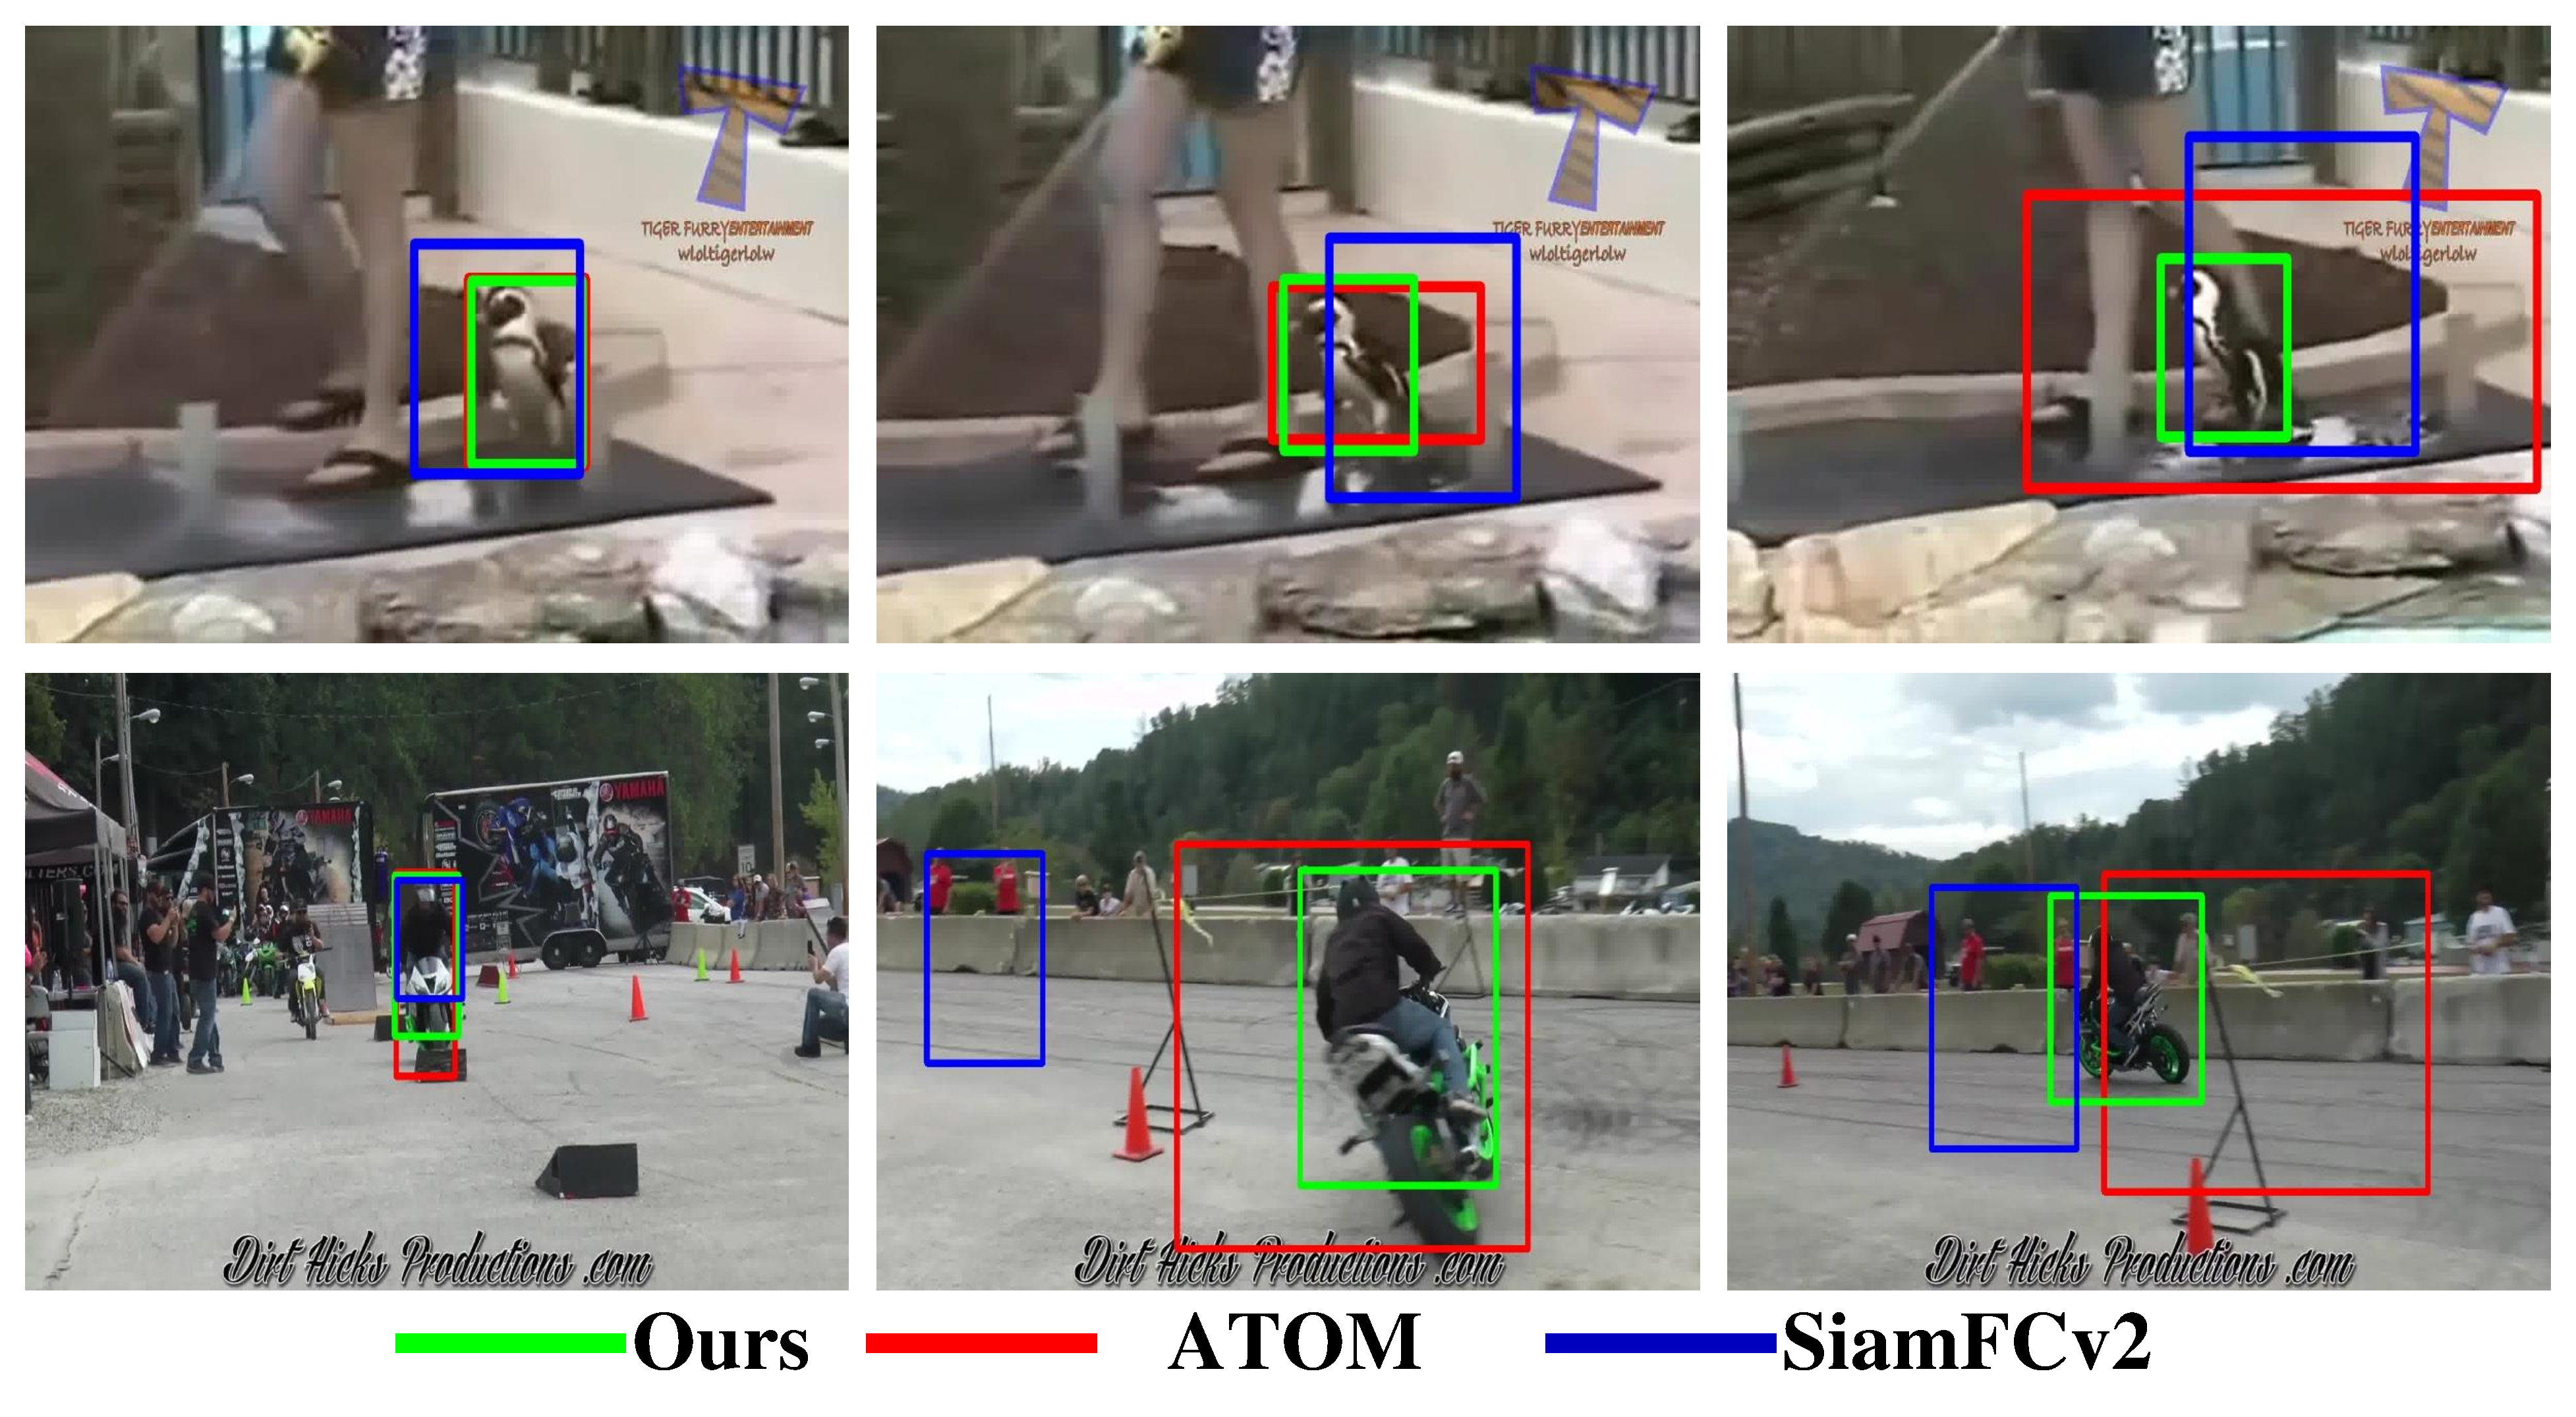
\includegraphics[width=1.0\textwidth]{Img/MTP/got10k/visulization2.pdf}
    \caption{本章提出的方法与跟踪器 ATOM \cite{danelljan2019atom} 和 SiamFCv2 \cite{SiamFC} 的比较。示例帧来自 GOT-10k \cite{GOT-10k} 测试集。}
    \label{fig:MTP_vis1}
\end{figure}

在本章中,我们表明视觉目标跟踪中具有挑战性的模型自适应任务可以通过简单地在孪生网络中操纵模板图像的像素来实现。给定一个视觉目标跟踪器,本章提出的算法使用第一帧中的目标真实标注框,仅在几次梯度下降迭代中修改模板像素。对于不包含在离线训练集中的目标,我们认为对模板图像像素进行微小修改可以改善离线训练的孪生网络的预测结果。我们使用对抗样本生成方法来实现此目的,因为对抗样本生成方法通常用于略微修改输入图像,从而对网络的预测结果产生影响。我们与对抗性样本生成的目的不同,因为后者旨在使网络预测变得更糟,而我们希望孪生网络的预测更好。本章提出的模型自适应方法可以与各种孪生跟踪器(如 SiamFC ++ \cite{SiamFC++})集成。在利用自适应信息提高跟踪性能的同时,孪生网络的参数保持不变,以保留离线训练的嵌入空间的表示能力。我们在 4 个视觉目标跟踪基准数据集上进行了全面的实验:VOT2018 \cite{kristan2018sixth}、TrackingNet \cite{muller2018trackingnet}、GOT-10k \cite{GOT-10k} 和 OTB2015 \cite{OTB}。本章提出的目标跟踪算法取得了较好的跟踪性能,同时以超过 80 FPS 的速度运行(见图 \ref{fig:MTP_vis})。
\section{相关工作}
模型更新是传统目标跟踪算法中的重要一环。然而,主流的孪生跟踪器通常采用离线训练的网络而不进行模型更新。由于没有在线学习,这些方法往往难以应对目标的表观变化和近似物体的干扰。
% UpdateNet
孪生网络跟踪器的基本原理是将目标表观模板的特征表示与测试帧中搜索区域的特征表示进行匹配。目标模板和搜索区域的特征是通过在大型数据集上离线训练的深度神经网络获取的。这种训练策略可以为跟踪任务提供出色的视觉描述符。在原始的孪生网络跟踪器 \cite{SiamFC} 中,目标模板在第一帧中初始化,然后在其余视频中保持固定。然而,目标表观的更改通常很大,不更新模板可能导致跟踪器过早失效。因此,使模型适应当前目标表观很重要。近年来,有一些算法尝试在孪生网络中进行模型更新。在文献 \cite{zhu2018distractor} 中,Zhu 等人提出使用简单的线性插值来更新每帧中的模板:
\begin{equation}
\widetilde{T}_{i}=(1-\gamma) \widetilde{T}_{i-1}+\gamma T_{i}.
\end{equation}
其中 $i$ 是帧的索引,$T_{i}$ 是仅使用当前帧计算的新模板样本,$\widetilde{T}_{i}$ 是累积的模板。通常,假设目标的表观在连续的帧中平滑且一致地变化,更新率 $\gamma$ 通常设置为较小的固定值(例如 $\gamma = 0.01$)。在孪生网络跟踪器中,$T$ 是由全卷积特征提取器从特定帧提取的目标表观模板。尽管模板平均提供了一种整合新表观的简单方法,但它也具有几个严重的缺点:

\begin{itemize}
\item 该方案对每个视频都采用恒定的更新速率,然而受多种因素(例如摄像机运动)的影响,不同视频的更新必要性不同。即使在同一视频中,目标模板所需的更新率也可能在不同时间中动态变化。
\item 更新率在模板的所有空间位置和所有通道上也是恒定的。然而在部分遮挡情况下,需要更新的仅仅是模板的一部分。
\item 跟踪器无法从漂移中恢复。部分原因是由于该方案无法访问初始表观模板 $T_{0}$,而初始表观模板 $T_{0}$ 是最可靠的模板。
\item 模板更新仅限于先前表观模板的简单线性组合。该策略限制了更新机制的灵活性,而这在目标经历复杂表观变化时非常重要。更复杂的模板特征组合功能可能有利于改善跟踪结果。
\end{itemize}

为了解决这些问题,在文献 \cite{Zhang_2019_ICCV} 中,Zhang 等人提出通过学习来对目标模板进行更新。学习的更新策略利用目标和图像信息。在该算法中,更新后的模板是根据以下内容计算的:(1)真实目标的初始模板,(2)所有先前帧的累积模板,以及(3)当前帧中预测的目标特征模板。因此,新的累积模板包含目标当前表观的有效历史信息,因为它会使用最新信息不断更新,同时由于使用了初始目标表观而增强了鲁棒性。具体而言,上述模板更新算法卷积神经网络 UpdateNet 来实现。这是一个轻量卷积神经网络,可以与任何孪生跟踪器结合使用,以增强其在线更新能力,同时保持跟踪器的跟踪效率。
%此外,学习有效的模板更新的细微差别非常复杂,并且足够自适应以处理大量的跟踪情况。
在文献 \cite{DiscriminativeAnd} 中,Zhou 等人提出了一个基于注意力机制的在线更新模块,可以充分利用背景信息为孪生目标跟踪网络提取特定于目标的特征。具体而言,作者提出通过分数融合使用特定于目标的特征进行判别性学习,以帮助孪生网络处理近似物体和背景噪音的干扰。此外,作者提出通过模板更新使用特定于目标的特征提高其鲁棒性,以应对目标形变、旋转和光照变化等情况。该在线更新模块可以与各种孪生跟踪器集成在一起,而无需进行重新训练。%Discriminative and Robust Online Learning for Siamese Visual Tracking
在文献 \cite{FCOT} 中,Cui 等人为分类和回归分支设计提出了统一的全卷积架构(FCOT)。这种简单的跟踪方法不仅可以进行有效的训练和部署,还可以在两个分支上进行在线学习,以进行准确而强大的跟踪。具体而言,作者设计了一个回归模型生成器来在线优化回归模型,从而使回归分支能够有效处理目标形变,从而获得更精确的跟踪结果。此外,作者为分类分支设计了多尺度预测策略,以处理近似目标混淆的问题。通过从粗到精的融合,可以提高跟踪方法的精确性和鲁棒性。 %https://arxiv.org/pdf/2004.07109.pdf
在文献 \cite{TGGAN} 中,为了避免漂移问题并执行在线自适应,Guo 等人使用条件 GAN 架构 \cite{cGAN} 来学习目标的通用表观分布。在跟踪阶段,我们使用学习到的 GAN 生成器生成目标模板。生成器将第一帧中的真实目标模板和随机矢量作为输入,并输出生成的目标模板。生成的模板被真实目标模板约束,因此不会漂移。同时,生成的模板可以模拟目标可能产生的表观变化。跟踪时,选择最适合当前目标表观的生成模板。通过这些策略,可以在线更新目标模板,同时避免漂移。%Generating Reliable Online Adaptive Templates for Visual Tracking

\section{自适应信息增强的视觉目标跟踪算法}
在本节中,我们通过直接操纵模板像素为孪生跟踪器提供一种新的模型自适应方法。我们首先回顾与基于模板匹配的主流跟踪器的跟踪过程。遵循文献 \cite{Danelljan_2020_CVPR},我们将目标跟踪形式化为基于置信度的回归问题,给定一个输出——输入对 $(y,x)$,该问题学习函数 $s_\theta:\mathcal{Y\times X\rightarrow \mathbb R}$,并预测标量置信度得分 $s_\theta(y,x)\in\mathbb R$。算法的最终预测 $f(x)=y^*$ 如下:
\begin{equation}
    f(x) = \arg\max_{y\in \mathcal Y}s_\theta (y,x),
\end{equation}
其中 $x$ 是输入图像。$y$ 通常表示目标的 2D 位置坐标。当前,有两种主流的基于模板匹配的跟踪框架:判别相关滤波器(discriminative correlation filter,DCF)方法和孪生跟踪方法。

基于 DCF 的方法在跟踪过程中训练循环相关滤波器 $w_{\theta}$ 来预测目标置信度得分:
\begin{equation}
    s_\theta(y,x)=(w_\theta \star \phi(x))(y),
    \label{equ:dcf}
\end{equation}
其中 $\phi(x)$ 是从搜索图像 $x$ 中提取的特征。

与 DCF 相比,孪生跟踪器采用双流体系结构。一个流根据模板图像 $z$ 提取目标的特征 $\phi_\theta(z)$,该模板图像是根据真实边界框从第一帧裁剪而来的。另一个流接收较大的搜索图像 $x$ 作为输入,并输出搜索特征 $\phi_\theta(x)$。这两个输出进行互相关以预测目标置信度得分:
\begin{equation}
    s_\theta(y,x)=(\phi_\theta(z) * \phi_\theta(x))(y).
    \label{equ:siamese}
\end{equation}

基于 DCF 的跟踪器和孪生跟踪器都具有利用大规模视觉目标跟踪数据集来训练特征提取器 $\phi(\cdot)$ 或嵌入网络 $\phi_{\theta}(\cdot)$ 的优势。因此,可以增强特征在目标跟踪任务上的表示能力。

与孪生跟踪器不同,DCF 利用目标模板图像学习滤波器 $w_\theta$,以将其与背景区分开。
尽管使用了循环相关运算提高了跟踪效率,但由于边界效应和复杂的优化使 DCF 无法在计算速度和跟踪性能之间做出良好的权衡。孪生跟踪器在这方面做得更好,然而在互相关中学习到的相似性度量对于未包含在离线训练集中的目标不一定是可靠的,从而导致泛化性较差。

在本章中,我们旨在设计一种新的孪生跟踪方法,该方法可以像基于 DCF 的跟踪器一样充分利用当前视频的特定信息进行模型调整,尽管其中的目标可能并不包含在离线训练时使用训练集中。我们通过利用第一帧中的注释信息执行模型自适应调整来实现这一目的。

注意等式 \ref{equ:dcf} 和等式 \ref{equ:siamese} 之间存在相似之处,主要区别在于进行相关计算的核:DCF 的核是在线学习的 $w_{\theta}$ ,而孪生网络的核是 $\phi_\theta(z)$。为了使孪生网络具有模型自适应能力,我们需要使用当前视频的第一帧标注信息来自适应调整 $\phi_\theta(z)$。调整 $\phi_\theta(z)$ 有两种设计选择:更改 $\phi_\theta(\cdot)$ 或更改 $z$。但是,更改 $\phi_\theta(\cdot)$ 可能会导致繁琐的元学习设置,难以确保离线训练的嵌入空间 \cite{ROAM, DBLP:conf/aaai/JungYNCH20}的特征表示能力。相反,我们的解决方案是以简单的方式通过更改 $z$ 来执行孪生跟踪器的模型自适应,即在第一帧使用目标真实标注信息仅在几次梯度下降迭代中修改模板像素。与当前的孪生跟踪模型自适应方法相比,该方法具有以下优点:

\begin{itemize}
\item 首先,我们不修改孪生网络的参数,从而保留离线训练的嵌入空间的表示能力。
\item 其次,与旨在合并先前帧目标特征的模板更新方法 \cite{zhu2018distractor, Zhang_2019_ICCV} 不同,我们专注于在第一帧使用目标真实标注信息进行初始自适应。
\item 最后,在不改变基线跟踪器整体架构的情况下,我们的模型自适应方法是即插即用。
\end{itemize}

在下一节中,我们将展示如何使用对抗样本生成方法来执行用于模型自适应的模板像素操纵。

\subsection{操纵模板像素以进行模型自适应}
乍看之下,模型自适应任务与对抗样本生成任务之间可能存在矛盾,因为这两个任务具有不同的目的。对抗样本 \cite{kurakin2017adversarial} 是对输入数据进行微小修改后的样本,目的是对机器学习系统进行攻击,导致机器学习模型做出错误的预测。然而,模型自适应的目的是在第一帧中充分利用注释信息,以提高当前视频的跟踪性能。接下来,我们将指出这两个任务之间存在一些相似之处,并且我们可以利用对抗样本生成方法来执行模型自适应任务。

在介绍提出的方法之前,我们首先回顾流行的对抗样本生成方法。生成对抗图像 $I^{adv}$ 的最简单方法之一是通过线性化干净图像的 $L_{\infty}$ 邻域中的损失函数,并使用以下闭式方程进行求解 \cite{FGSM}:
\begin{equation}
    I^{adv} = I + \epsilon \text{ sign} \bigl( \nabla_I L(I, y_{true})  \bigr),
\end{equation}
其中 $I$ 是输入图像,像素值是 [0,255] 范围内的整数。 $y_{true}$ 是图像 $I$ 的真实标签。给定图像 $I$ 和标签 $y$,$L(I, y)$ 是用于攻击神经网络的损失函数。$\epsilon$ 是超参数。扩展上述方法的一种直接方案是,以较小的步长迭代应用该公式,并在每次迭代之后裁剪中间结果的像素值,以确保位于原始图像的 $\epsilon$ 邻域中。这导致在 \cite{kurakin2017adversarial} 中引入了基本迭代方法(BIM):
\begin{equation}
    \begin{gathered}
        I_0^{adv} = I, \\
        I_{N+1}^{adv} = Clip_{I,\epsilon}\{I_N^{adv}+\alpha \text{ sign}(\nabla_I L(I_N^{adv},y_{true}))\},
    \end{gathered}
\end{equation}
其中 $Clip_{I, \epsilon} \left\{ I' \right\}$ 用于对图像 $I'$ 进行逐像素裁剪,从而保证结果在原始图像 $I$ 的 $L_{\infty}$ $\epsilon$ 邻域内。
BIM 可以进行扩展以攻击特定的期望目标类别 \cite{kurakin2017adversarial}:
\begin{equation}
    \begin{gathered}
        I_0^{adv} = I,\\
        I_{N+1}^{adv} = Clip_{I,\epsilon}\{I_N^{adv}-\alpha \text{ sign}(\nabla_I L(I_N^{adv},y_{target}))\}.
    \end{gathered}
    \label{equ:itcm}
\end{equation}
等式 \ref{equ:itcm} 表明,仅需进行几次梯度下降迭代操作对输入图像的像素进行修改,就可以将网络的预测更改为特定类别 $y_{target}$。请注意,我们的目的是在第一帧中修改模板图像的像素,以使预测更接近于真实边界框。因此,我们可以使用等式 \ref{equ:itcm} 进行一些修改,用于对孪生网络进行模型自适应:
\begin{equation}
    \begin{gathered}
        z_0 = z,\\
        z_{N+1} = Clip_{z,\epsilon}\{z_N -\alpha \text{ sign}(\nabla_z L(z_N,y_{bb}))\},
    \end{gathered}
    \label{equ:adaptaion}
\end{equation}
其中 $z$ 是第一帧中的模板图像,而 $y_{bb}$ 是根据真相边界框生成的孪生跟踪器的标签。在下一节中,我们将介绍配备了所提出的模型自适应模块的跟踪器的整体跟踪过程。

%%%%%%%%%%%%%%%%
\begin{table}[t]
\caption{在视觉目标跟踪数据库 OTB2015 上进行比较。FPS:每秒帧数。跟踪器速度在 NVIDIA RTX 2080Ti GPU 上进行测试。}
\setlength{\tabcolsep}{3pt}
\begin{center}
\begin{tabular}{r c c c c c c}
\toprule
Trackers & ECO & MDNet & SiamRPN++ & ATOM & SiamFC++\_G & Ours \\
\midrule
Success & 70.0 & 67.8  & 69.6      & 66.9      & 68.3       & 69.7 \\
FPS     & 8    & 1     & 35        & 30       & 90         & 82  \\
\bottomrule
\end{tabular}
\end{center}
\label{table:otb}
\end{table}
%%%%%%%%%%%

%%%%%%%%%%%%%%%%
\begin{table}[t]
\centering
\caption{在 TrackingNet 测试数据集上对精确度,标准化精确度和成功率的比较。}
\begin{tabular}{l c c c}
\toprule
Method   &  Prec.   &  Norm. Prec. & Succ.  \\
\midrule
Ours  &  70.6&  81.7 &74.9 \\
SiamFC++\_G& 70.5 & 80.0 & 75.4 \\
SiamFC++\_A  & 64.6 & 75.8 & 71.2 \\
ATOM              & 64.8 & 77.1 & 70.3 \\
SiamRPN++&  69.4 & 80.0 &73.3 \\
MDNet	 &  56.5&  70.5 &60.6 \\
ECO	 &  49.2&  61.8 &55.4 \\
SiamFC	 &  51.8&  65.2 &55.9 \\
\bottomrule
\end{tabular}
\label{tabel:trackingnet}
\end{table}
%%%%%%%%%%%

%%%%%%%%%%%%%%%%%%%%%%%%%%%%%%%
\subsection{跟踪框架}
所提出的模型自适应方法以即插即用的方式与 SiamFC++ 跟踪器 \cite{SiamFC++} 集成在一起。 SiamFC++ 基于 SiamFC \cite{SiamFC},并根据 \cite{SiamFC++} 中提出的一些准则逐步完善。原始 SiamFC++ 网络的输入由从第一帧裁剪的模板图像 $z_0$ 和从第 $i$ 帧裁剪的搜索图像 $x_i$ 组成。但是,我们希望执行模板像素操纵,以便在对输入对 $(z_0, x_0)$ 进行 $N$ 步像素更新获得 $z'$ 后,跟踪器在 $(z', x_i)$ 上表现良好。为此,我们首先在第一帧根据目标的真实标注框裁剪初始模板图像 $z_0\in\mathbb R^{3\times128\times 128}$ 和初始搜索图像 $x_0\in\mathbb R^{3\times289\times 289}$。
然后,将 $z_0$ 和 $x_0$ 发送到 SiamFC++ 网络以获得第一帧的跟踪预测。SiamFC++ \cite{SiamFC++} 中的跟踪损失计算如下:
\begin{equation}
    L = L_{\text{cls}} + L_{\text{quality}} + L_{\text{reg}},
\end{equation}
其中 $L_{\text{cls}}$ 是焦点损失 \cite{focal}。$L_{\text{quality}}$ 是用于质量评估的二进制交叉熵(BCE)损失。$L_{reg}$ 是边框回归的 IoU 损失 \cite{yu2016unitbox}。根据等式 \ref{equ:adaptaion},相对于模板 $z_0$ 的梯度用于生成 $z_1$。通过应用少数几次迭代可以获得更新的模板 $z'$(等式 \ref{equ:adaptaion})。请注意,模板图像仅使用给定序列的第一帧进行更新,并在整个跟踪过程中保持固定以确保稳定性。
后续跟踪过程与SiamFC++ 相同。

%%%%%%%%%%%%%%%%%%%%%
\section{实验评估与分析}

%%%%%%%%%%%%%
\begin{table}[t]
\caption{在不同数据库上的消融实验。}
\begin{center}
\begin{tabular}{c cc c}
\toprule
跟踪器 & 评价指标 & 基线方法 & 本章方法\\
\midrule
\multirow{1}{*}{OTB-15} 
& Success & 68.3 & 69.7\\
\midrule
\multirow{3}{*}{VOT-18}
& A   & 0.587 & 0.591 \\
& R   & 0.183 & 0.187 \\
& EAO & 0.426 & 0.438 \\
\midrule
\multirow{3}{*}{GOT} 
& SR\textsubscript{.50} &  0.737 & 0.748 \\
& SR\textsubscript{.75} & 0.464 & 0.475 \\
& AO & 0.607 & 0.617 \\
\midrule
\multirow{3}{*}{T-Net} 
& Prec.       & 70.5 & 70.6 \\
& Norm. Prec. & 80.0 & 81.7 \\
& Succ.       & 75.4 & 74.9 \\
\midrule
\multicolumn{2}{c}{FPS} & 90 & 82\\
\bottomrule
\end{tabular}
\end{center}
\label{tab:benchmark results}
\end{table}
%%%%%%%%%%%

%%%%%%%%%%%%%%%%%
\begin{figure}[t]
    \centering
    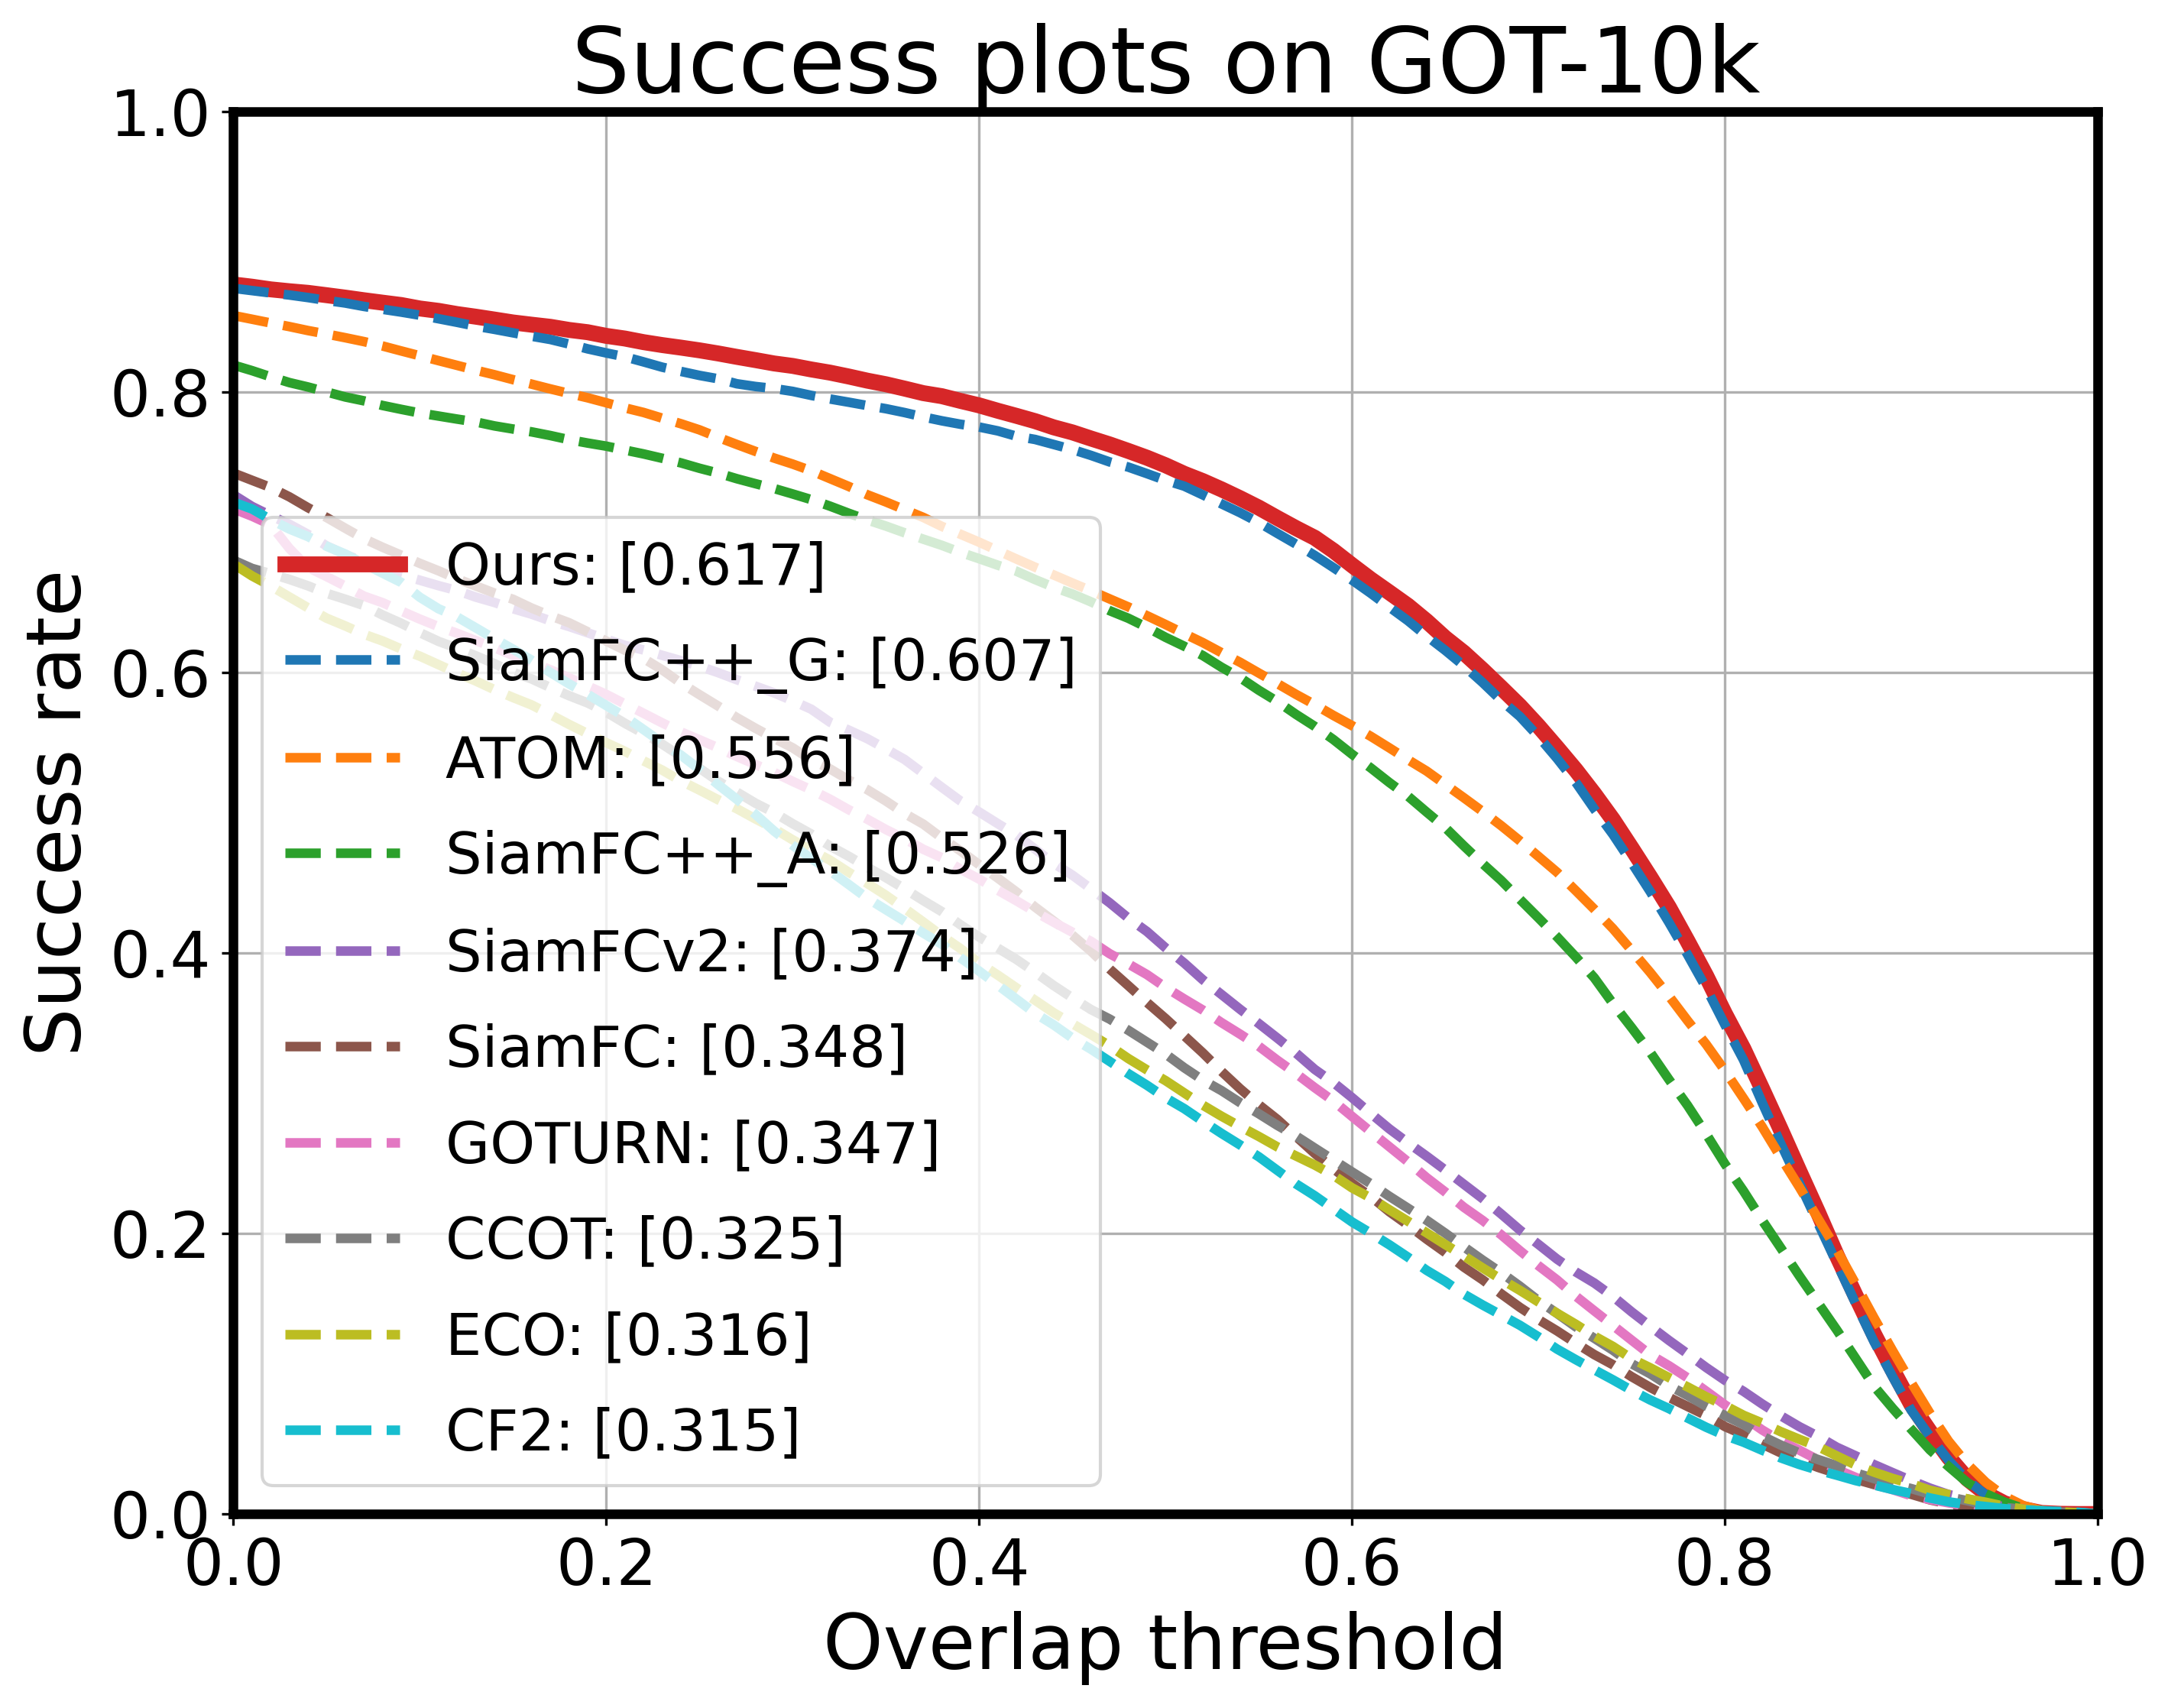
\includegraphics[width=0.75\textwidth]{Img/MTP/got10k/success_plot.png}
    \caption{将本章提出的跟踪器与其他跟踪器在 GOT-10k 测试集上进行比较。按平均重叠分数对跟踪器进行排名。}
    \label{fig:got10k}
\end{figure}
%%%%%%%%%%%%

\begin{figure}[p]
    \centering
    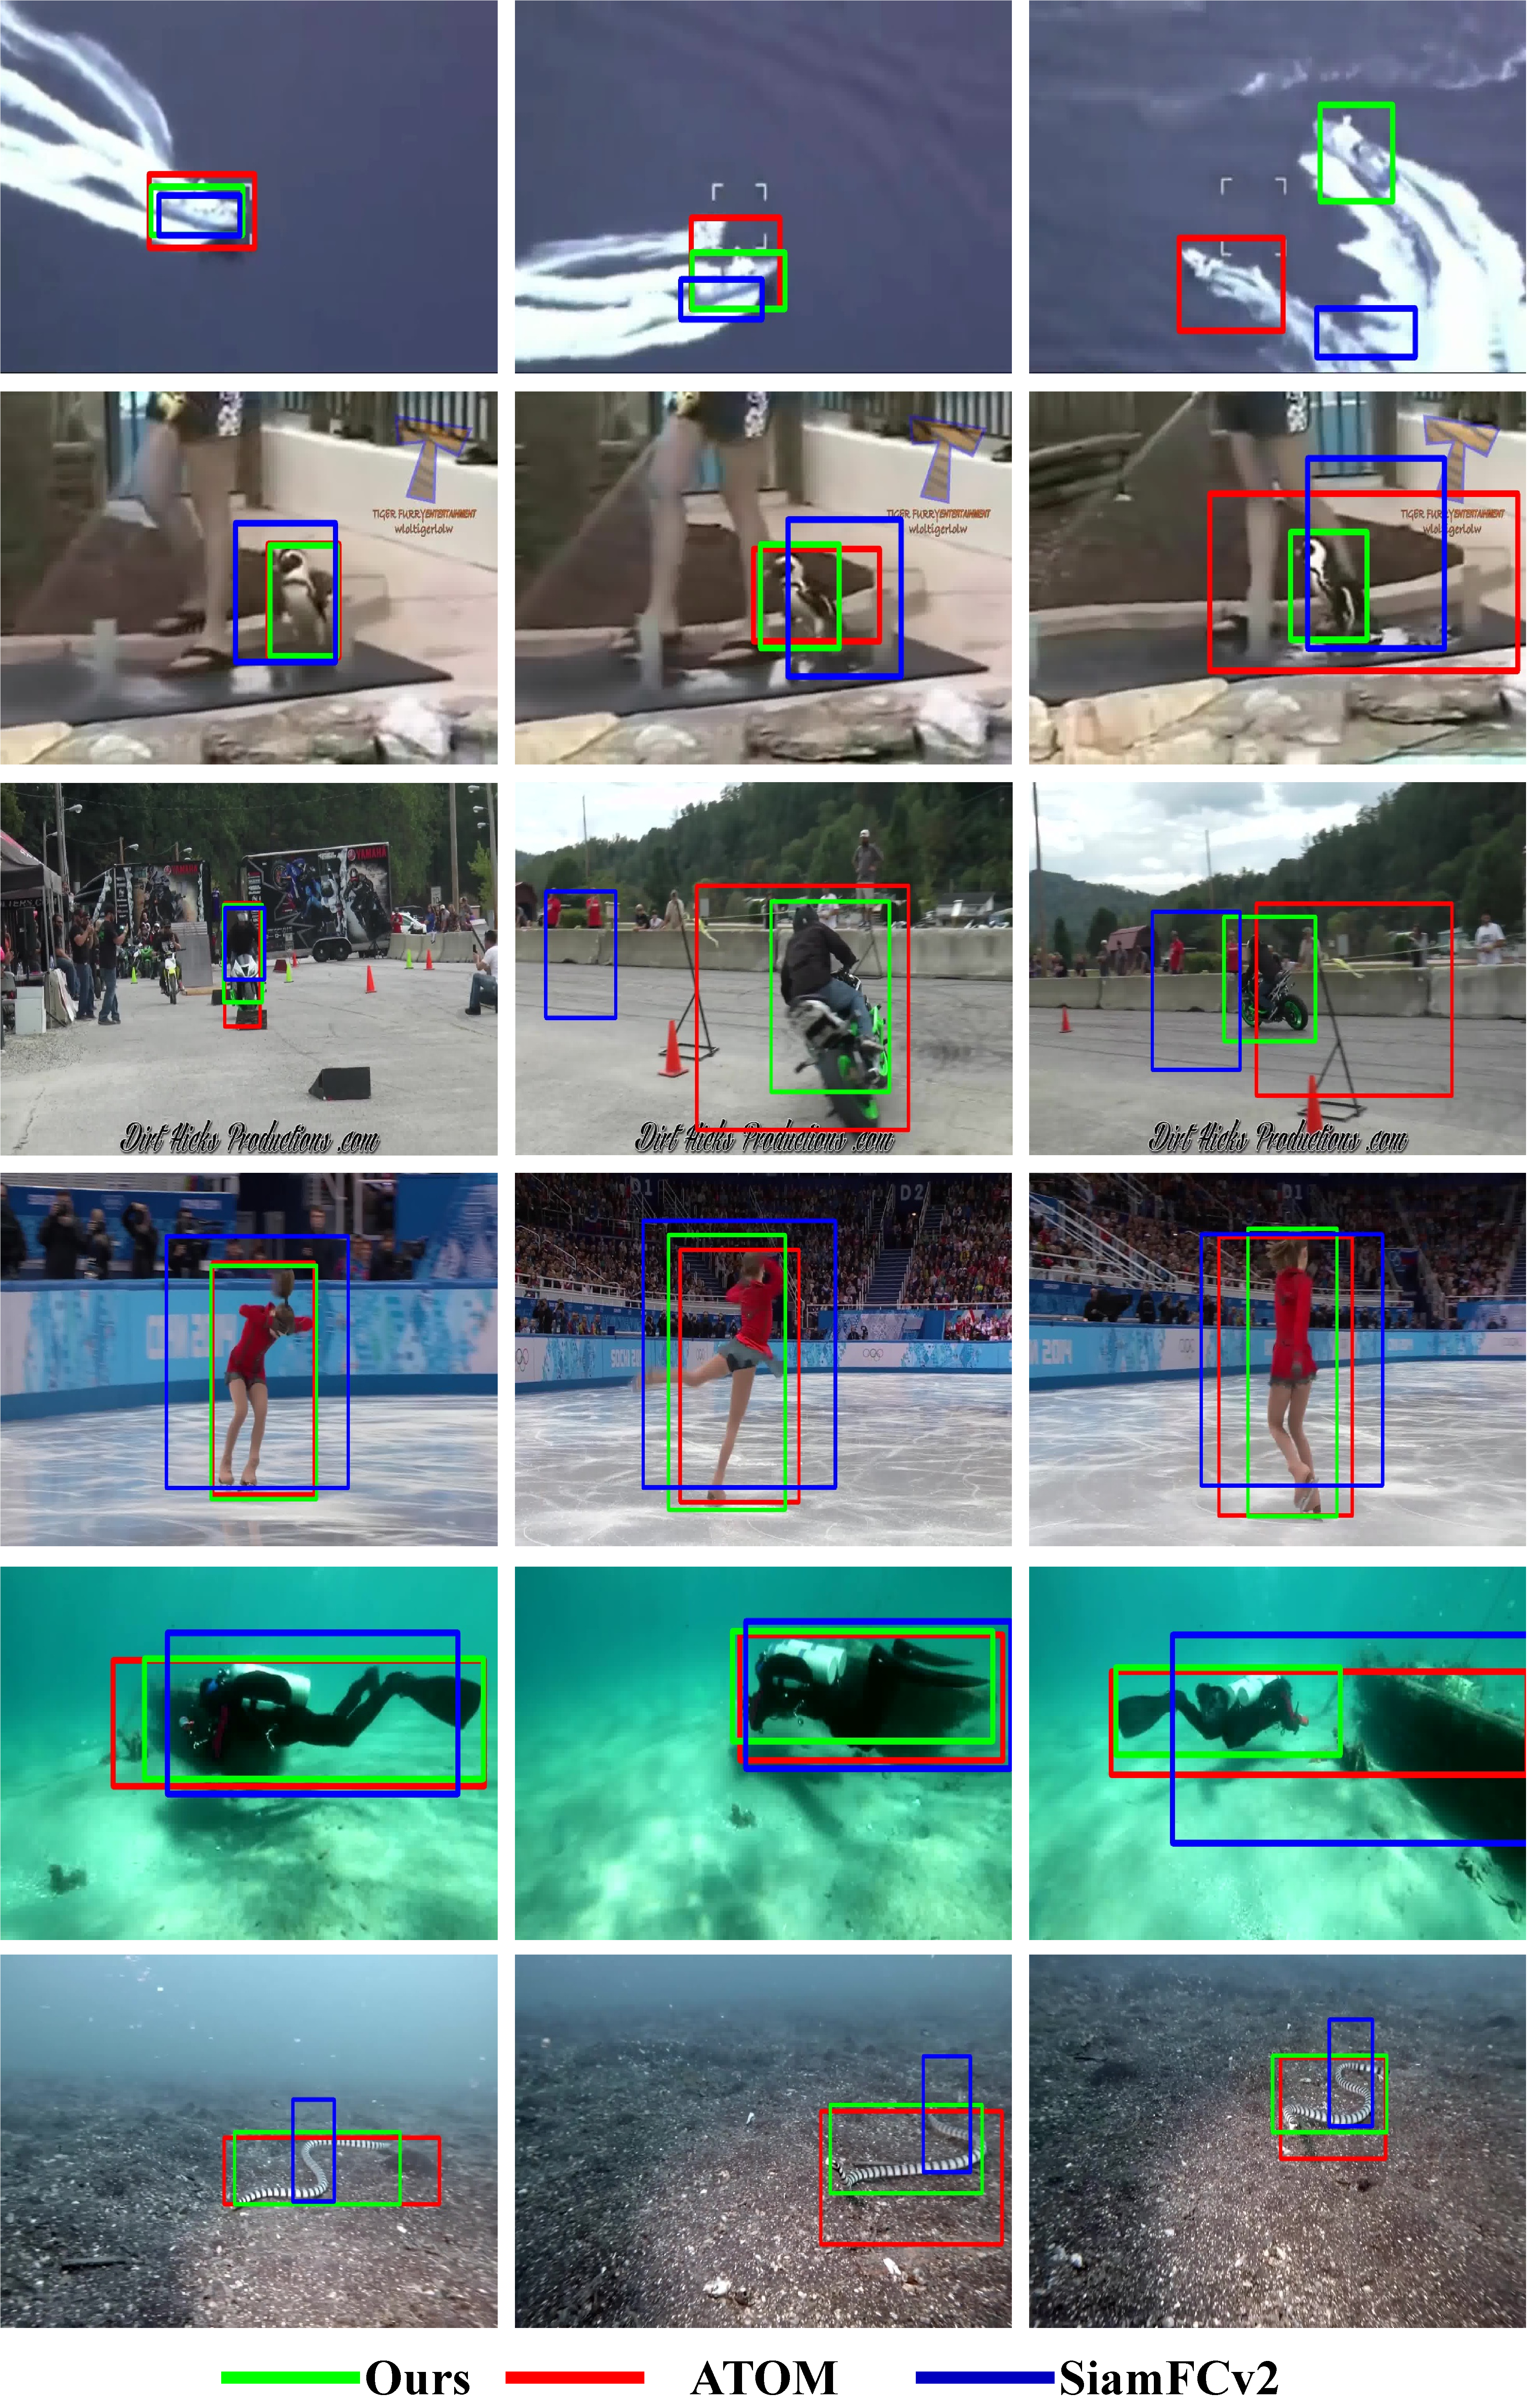
\includegraphics[width=0.99\textwidth]{Img/MTP/got10k/visulization.pdf}
    \caption{本章提出的跟踪器与 ATOM \cite{danelljan2019atom} 和 SiamFCv2 \cite{SiamFC} 的比较。示例帧来自 GOT-10k \cite{GOT-10k} 测试集。}
    \label{fig:MTP_vis}
\end{figure}

\begin{figure}[t!]
    \centering
    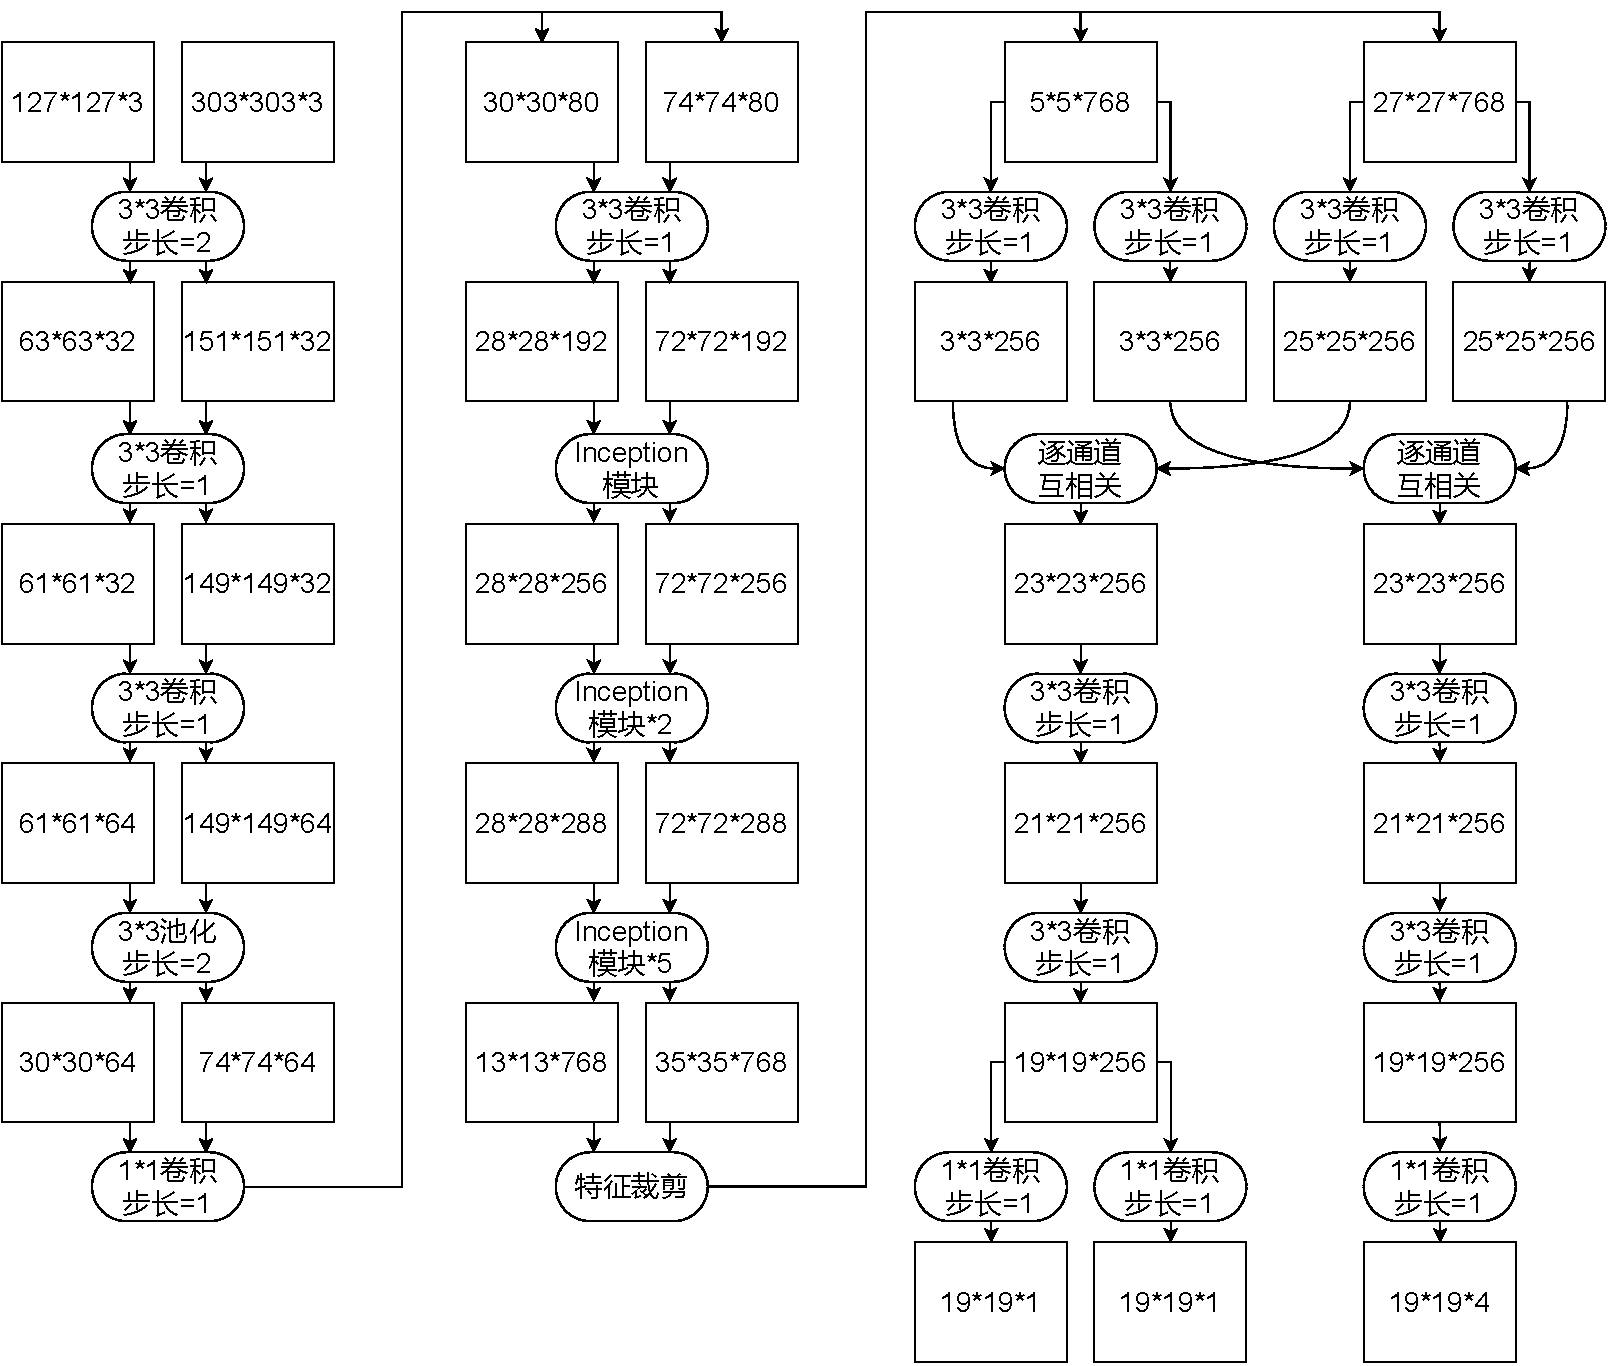
\includegraphics[width=0.99\textwidth]{Img/MTP/SiamFC++.pdf}
    \caption{网络结构参数示意图。}
    \label{fig:MTP_SiamFC++}
\end{figure}

\subsection{实验设置}
\textbf{网络架构设计}:本章所采用的基线孪生目标跟踪网络主要由四个子网络组成,分别是用于共享特征提取的主干网络,用于预测边框位置的回归子网络,用于判断目标出现可能性的分类分支,以及用于预测边框质量的质量评估分支。网络结构如图 \ref{fig:MTP_SiamFC++} 所示。主干网由 5 个卷积层和 8 个 Inception 块 \cite{GoogLeNet} 构成,可为模板图像和搜索图像提取高层语义信息,以提升跟踪精度。

\textbf{训练数据}:为了提高特征表示的泛化能力和判别力,同时避免在稀缺的跟踪数据上过度拟合,基线网络的离线训练数据集包括 ILSVRC-VID/DET \cite{VID}、COCO \cite{COCO}、YoutubeBB \cite{real2017youtube}、LaSOT \cite{LaSOT} 和 GOT-10k \cite{GOT-10k}。
其中,大规模视觉识别挑战赛(ImageNet Large Scale Visual Recognition Challenge,简称 ILSVRC)数据集包含超过 4000 个视频序列以及约 130 万个矩形框标注,具有较为丰富多样的视频场景分布。
COCO 数据集是一个大型的、丰富的物体检测、分割和字幕数据集。该数据集以场景理解为目标,主要从复杂的日常场景中截取,图像中的目标通过精确的分割进行位置的标定。图像包括 91 类目标,328000 幅图像和 2500000 个标签。
YoutubeBB 数据集是带有高质量单目标边框注释的大规模数据集,从 240000 段 YouTube 视频中提取大约 380000 个时长 15 秒至 20 秒的视频片段。所选择的视频大多以手持设备(如手机摄像头)拍摄,未进行编辑和后处理。所有视频片段标注有高精度的分类标签,并以 1 帧每秒的帧率进行人工边框标注。该数据集的目的是推动机器学习的进展,以促进视频理解。
LaSOT 数据集是一个具有高质量手动密集标注的对象跟踪数据集,包含 1400 个视频,每个序列平均 2512 帧。每一帧都经过仔细检查和手动标记,并在需要时对结果进行目视检查和纠正,从而生成大约 352 万个高质量的边界框标注。LaSOT 共包含 70 个类别,每个类别包含 20 个序列。
GOT-10k \cite{GOT-10k} 包括超过一万个视频片段,分为 563 类运动目标和 87 类运动模式,以尽可能覆盖现实情况中的各种挑战性模式,并带有超过 150 万个手动标记的边界框,从而可以对深度跟踪器进行统一训练和稳定评估。在 GOT-10k 采用的跟踪器评估协议中,训练集和测试集的物体类别是零重叠的。该协议避免了评估结果的偏差
上述数据集被广泛使用在最近提出的孪生网络跟踪算法 \cite{SiamRPN++,Wang2018SiamMask} 训练中。
对于视频数据集 VID、LaSOT 和 GOT-10k,从间隔小于 100 帧内抽取图像对。对于视频数据集 YoutubeBB,从间隔小于 5 帧内抽取图像对。对于图像数据集 COCO 和 ImageNetDet,生成负样本对作为训练样本的一部分,以增强模型区分近似目标的能力。在搜索图像上按均匀分布指定随机平移和缩放以进行数据增强。

\textbf{优化器参数设定}:对于基线网络的训练,使用动量为 0.9 的随机梯度下降(stochastic gradient descent,SGD)优化器对网络参数进行训练,并将权值衰减参数设置为 0.0005。
模型经过 20 个迭代周期的训练,每个迭代周期中图像对的数量为 300000 对。
主干网络中的参数在前 10 个迭代周期中被冻结,并从第 11 个迭代周期开始进行训练以避免过拟合。
模型的全局学习率为 $2\times 10^{-2}$。主干网络中参数的学习率为全局学习率的十分之一。
公式 \ref{equ:adaptaion} 中的参数 $\alpha$ 设为 0.05。

\textbf{测试阶段}:测试时,除利用自适应信息对模板像素进行调整外,不对基线网络进行任何更改。测试阶段的模型输出是一组带有置信度得分的边界框。根据边界框的尺度/长宽比变化以及距上一帧中预测目标的位置,对置信度得分进行惩罚,最后选择得分最高的边界框用于更新目标状态。

本章所提出的自适应信息增强的孪生网络跟踪器使用 PyTorch 在 Python 中实现,所有实验在装配有 Intel(R) Xeon(R) CPU E5-2630 v4 @ 2.20GHz
和 NVIDIA RTX 2080Ti GPU 的工作站上执行。本章提出的跟踪器在 NVIDIA RTX 2080Ti GPU 上以超过 80 FPS 的速度运行。

%%%%%%%%%%%%%%%%%
\begin{figure}[t]
    \centering
    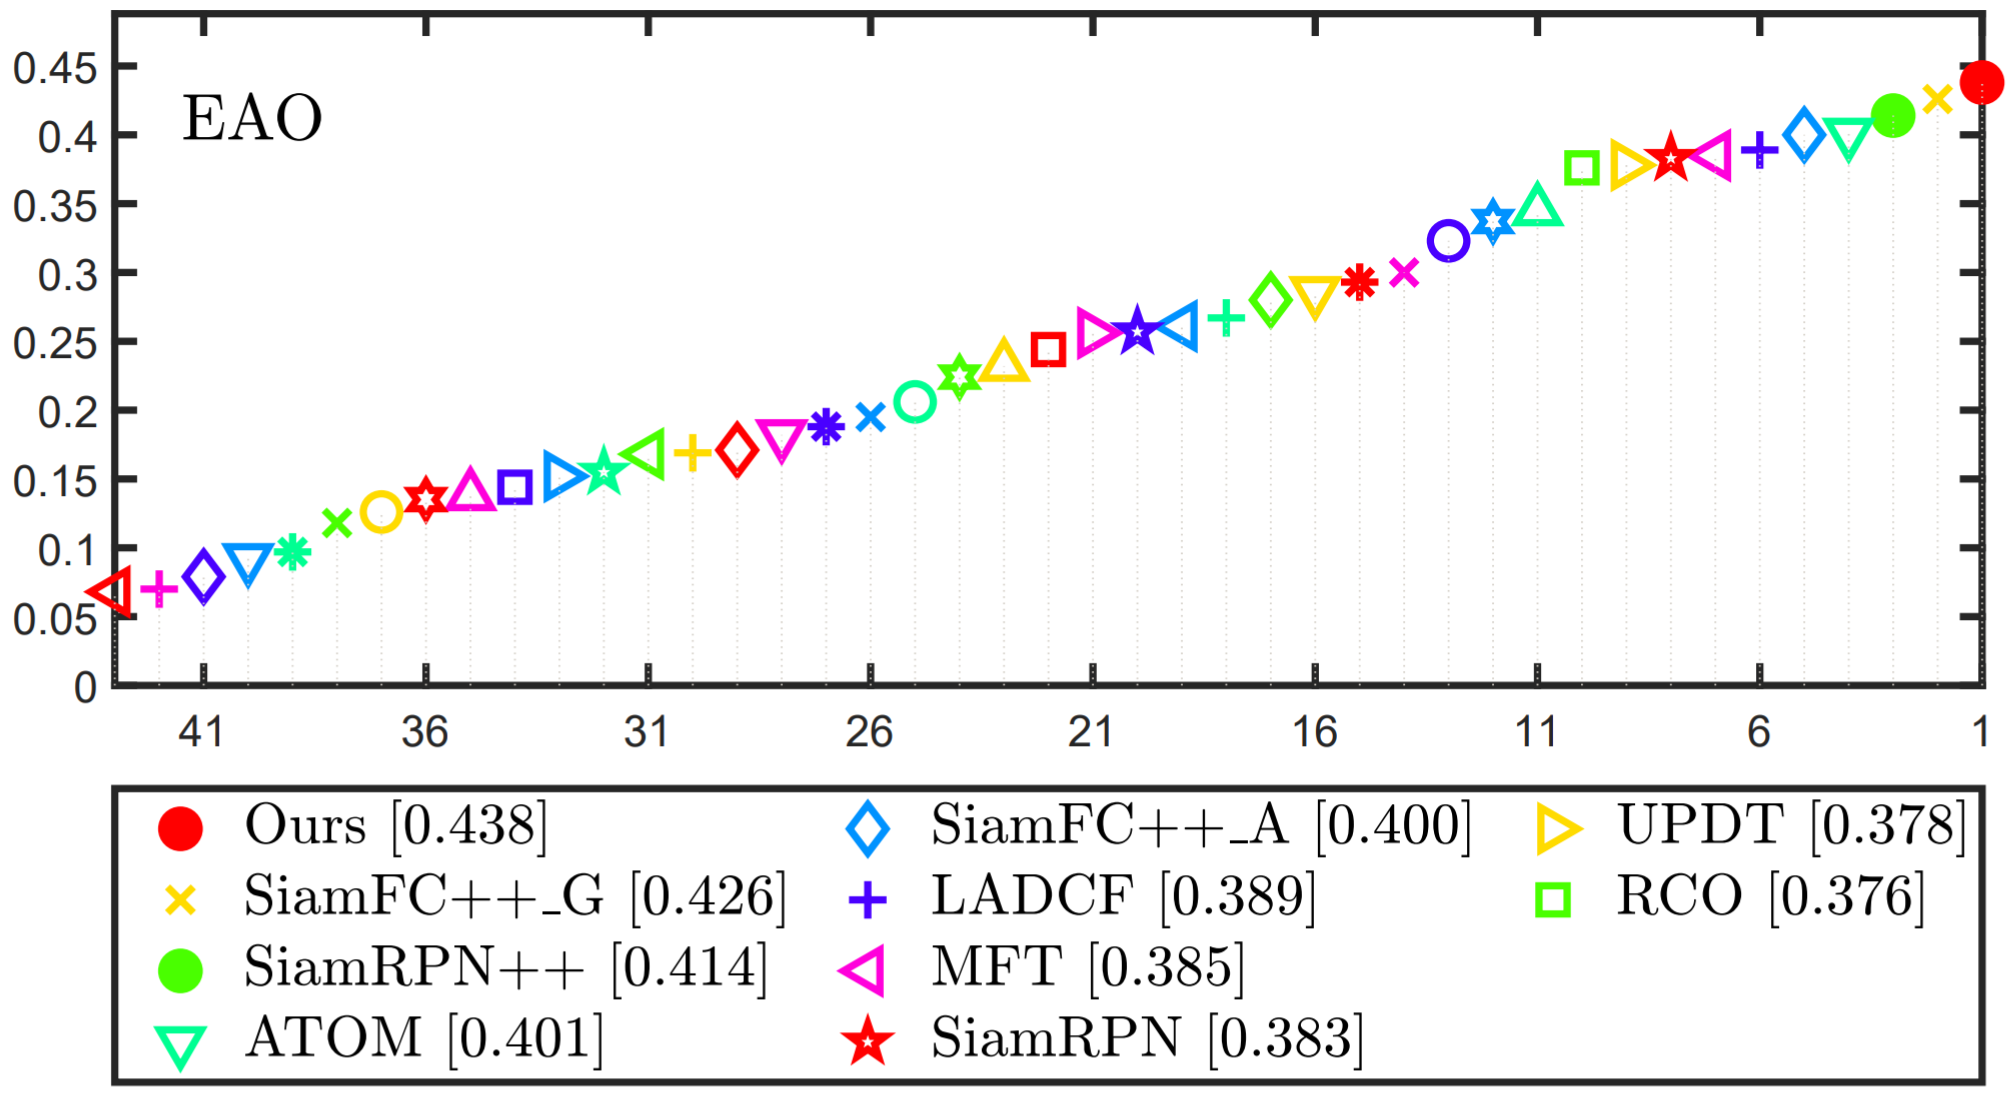
\includegraphics[width=1.0\textwidth]{Img/MTP/vot18/vot18_eao.png}
    \caption{预期平均重叠图。跟踪器根据 VOT2018 的预期平均重叠值从右到左排列。最右边的跟踪器是跟踪性能最好的跟踪器。}
    \label{fig:eao}
\end{figure}
%%%%%%%%%%%%


%%%%%%%%%%%%%%%%%%%%%%%%%%%%%%%%%%%%%
\subsection{与主流跟踪器的比较}

在本节中,我们将本章提出的方法与主流跟踪器在四个跟踪数据集上进行比较:OTB2015 \cite{OTB},VOT2018 \cite{kristan2018sixth},GOT-10k \cite{GOT-10k} 和 TrackingNet \cite{muller2018trackingnet}。具体来说,OTB2015 \cite{OTB} 包含 100 个序列,这些序列标记有不同的属性,用于深入分析跟踪性能。VOT2018 \cite{kristan2018sixth} 独特地应用了基于重置的方法,并挑选了 60 种序列对各种跟踪方案进行评估。GOT-10k \cite{GOT-10k} 和 TrackingNet \cite{muller2018trackingnet} 是最近提出的两个视觉目标跟踪数据集。它们在训练和测试集中涵盖了的各种目标类和场景。对于 GOT-10k,训练和测试集之间的目标类别没有重叠,从而可以有效评估跟踪其对目标类别的泛化能力。

\iffalse
\begin{figure*}[p]
\begin{center}
\subfloat[]{
	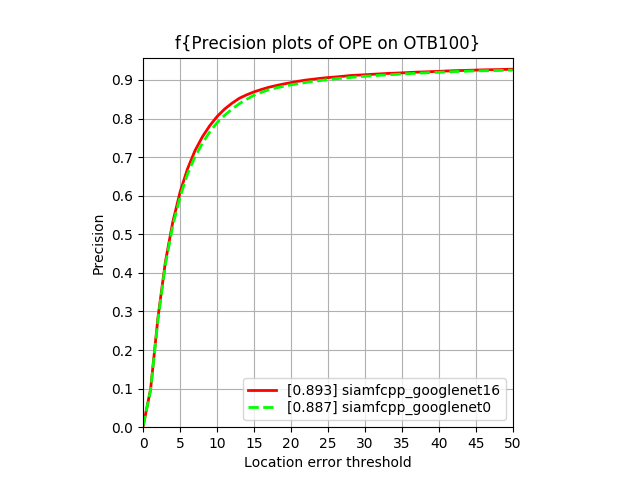
\includegraphics[width=0.33\textwidth]
	{Img/MTP/otb2015/precision_ALL.png}
}
\subfloat[]{
	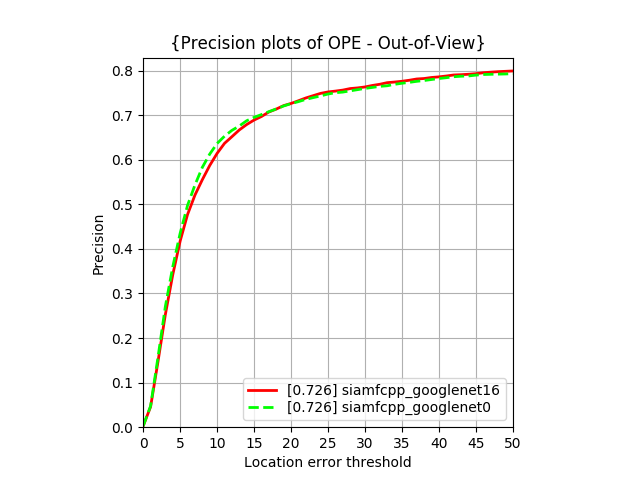
\includegraphics[width=0.33\textwidth]
	{Img/MTP/otb2015/precision_Out-of-View.png}
}
\subfloat[]{
	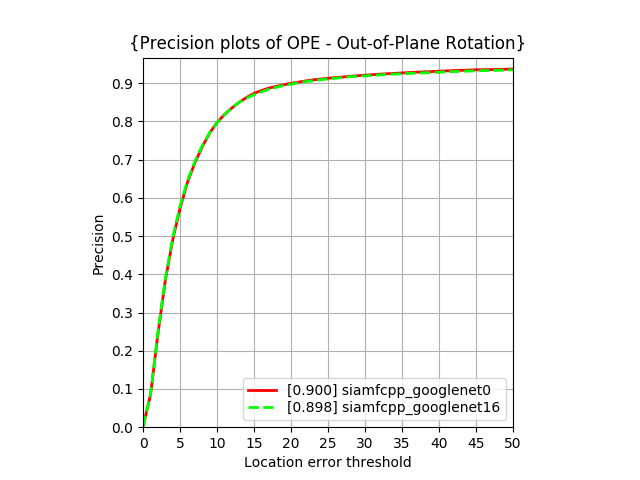
\includegraphics[width=0.33\textwidth]
	{Img/MTP/otb2015/precision_Out-of-Plane Rotation.png}
}\\
\subfloat[]{
	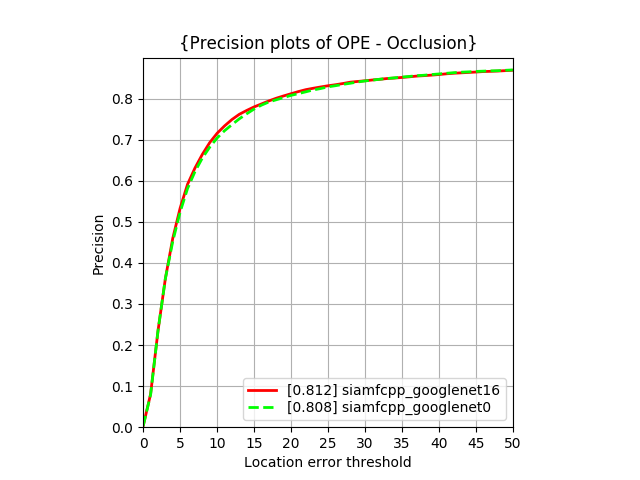
\includegraphics[width=0.33\textwidth]
	{Img/MTP/otb2015/precision_Occlusion.png}
}
\subfloat[]{
	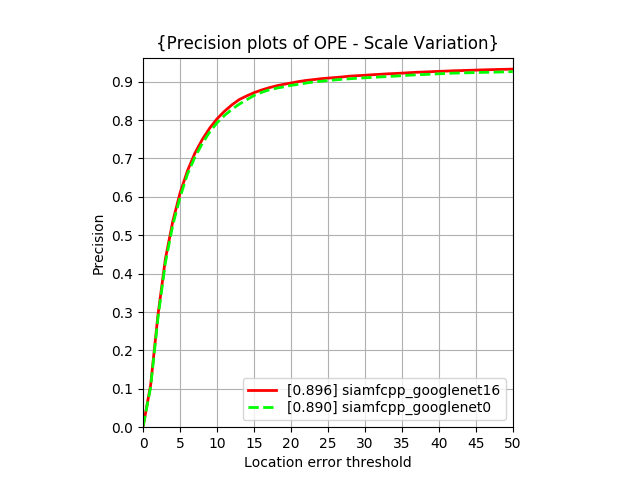
\includegraphics[width=0.33\textwidth]
	{Img/MTP/otb2015/precision_Scale Variation.png}
}
\subfloat[]{
	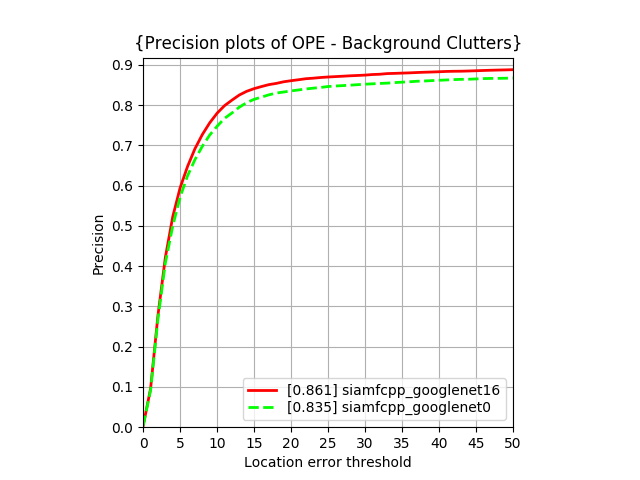
\includegraphics[width=0.33\textwidth]
	{Img/MTP/otb2015/precision_Background Clutters.png}
}\\
\subfloat[]{
	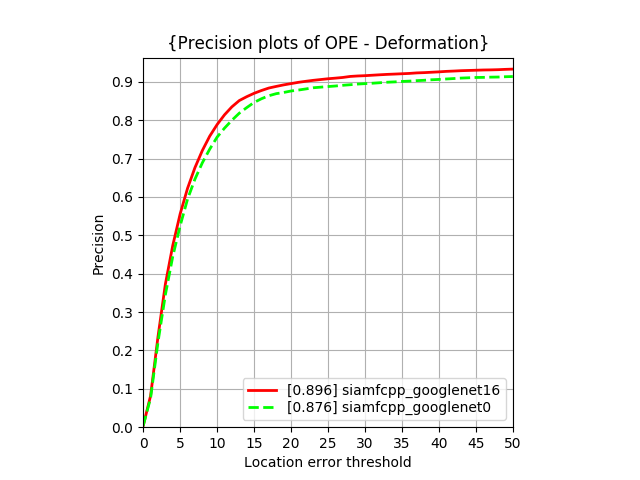
\includegraphics[width=0.33\textwidth]
	{Img/MTP/otb2015/precision_Deformation.png}
}
\subfloat[]{
	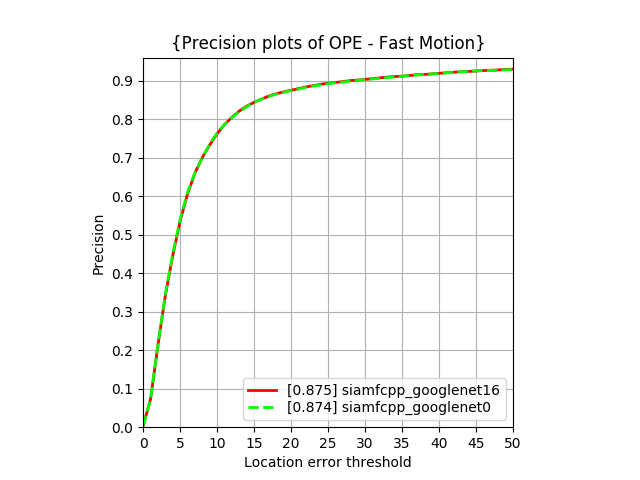
\includegraphics[width=0.33\textwidth]
	{Img/MTP/otb2015/precision_Fast Motion.png}
}
\subfloat[]{
	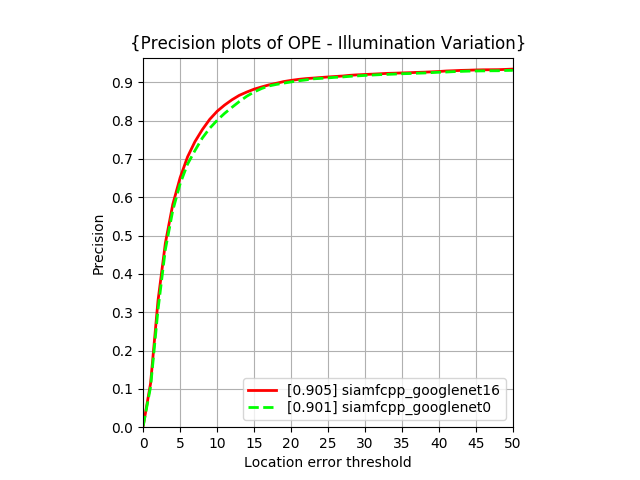
\includegraphics[width=0.33\textwidth]
	{Img/MTP/otb2015/precision_Illumination Variation.png}
}\\
\subfloat[]{
	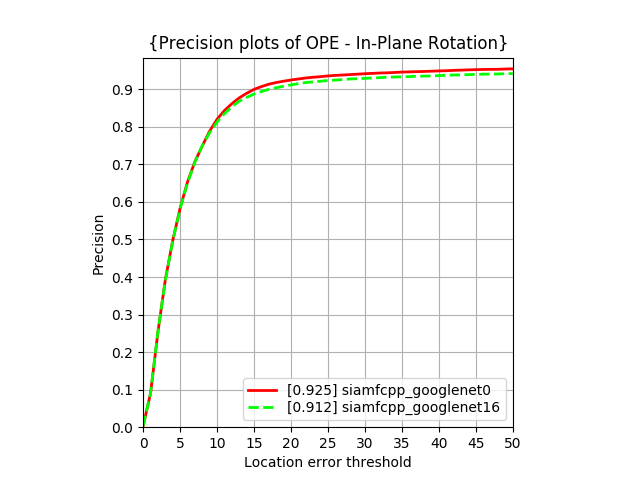
\includegraphics[width=0.33\textwidth]
	{Img/MTP/otb2015/precision_In-Plane Rotation.png}
}
\subfloat[]{
	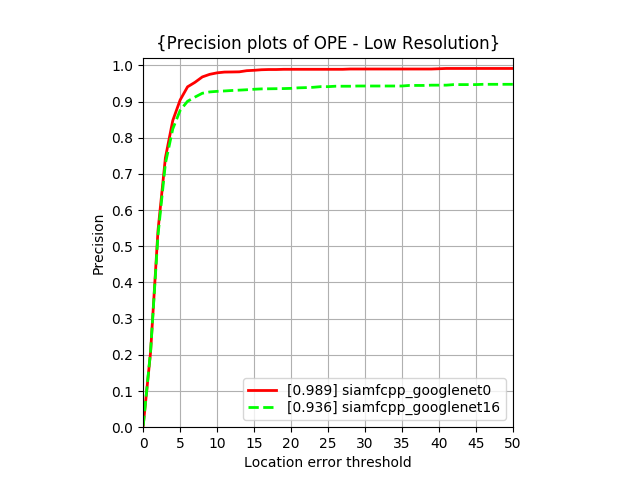
\includegraphics[width=0.33\textwidth]
	{Img/MTP/otb2015/precision_Low Resolution.png}
}
\subfloat[]{
	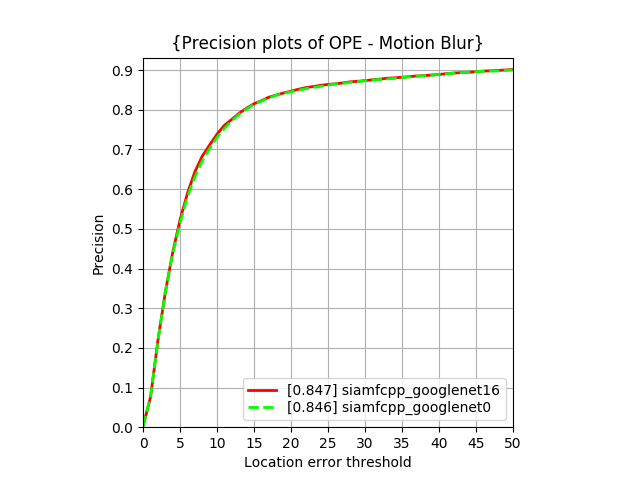
\includegraphics[width=0.33\textwidth]
	{Img/MTP/otb2015/precision_Motion Blur.png}
}
\end{center}
   \caption{OTB 各属性精度图。}
\end{figure*}

\begin{figure*}[p]
\begin{center}
\subfloat[]{
	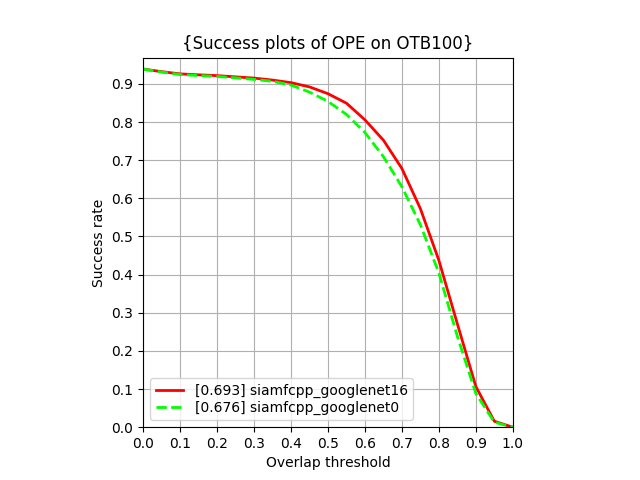
\includegraphics[width=0.33\textwidth]
	{Img/MTP/otb2015/success_ALL.png}
}
\subfloat[]{
	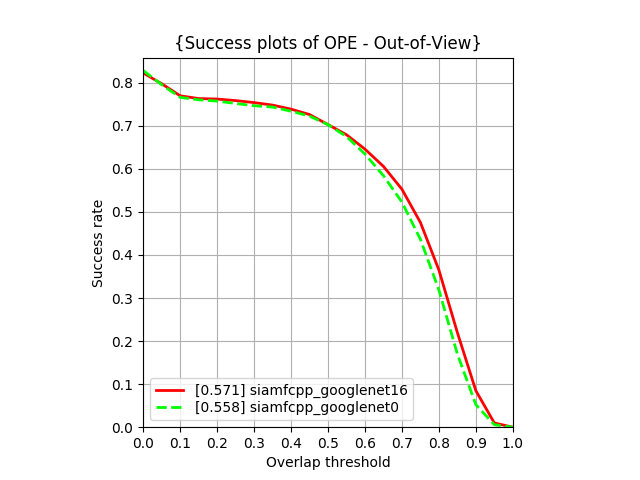
\includegraphics[width=0.33\textwidth]
	{Img/MTP/otb2015/success_Out-of-View.png}
}
\subfloat[]{
	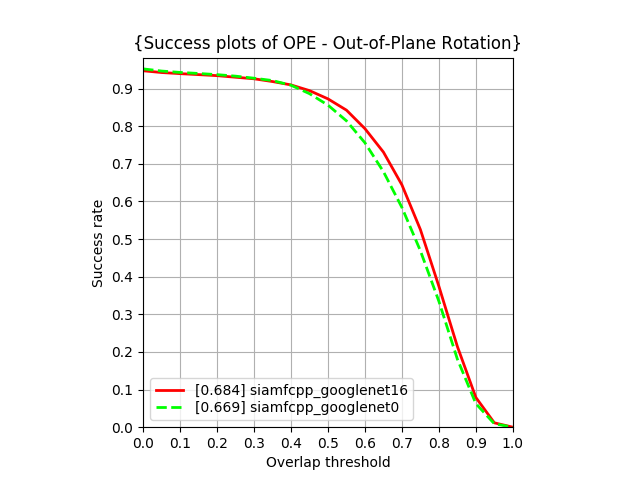
\includegraphics[width=0.33\textwidth]
	{Img/MTP/otb2015/success_Out-of-Plane Rotation.png}
}\\
\subfloat[]{
	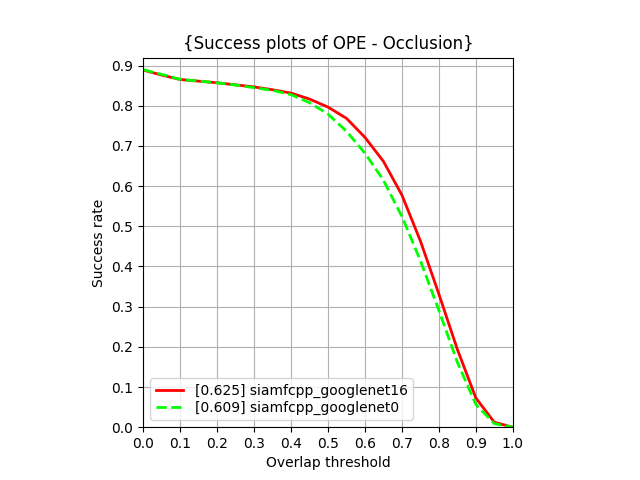
\includegraphics[width=0.33\textwidth]
	{Img/MTP/otb2015/success_Occlusion.png}
}
\subfloat[]{
	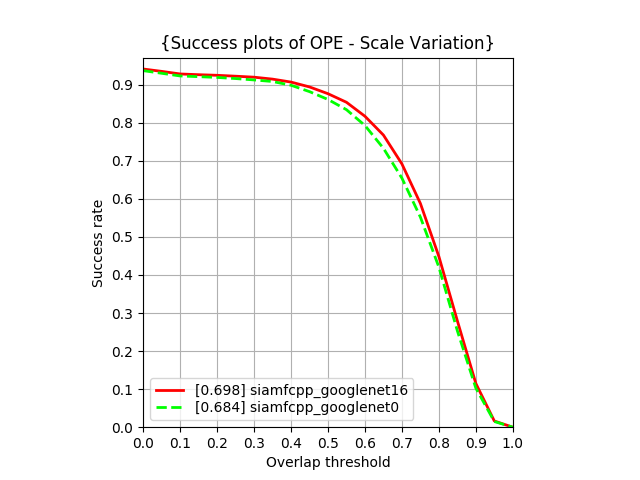
\includegraphics[width=0.33\textwidth]
	{Img/MTP/otb2015/success_Scale Variation.png}
}
\subfloat[]{
	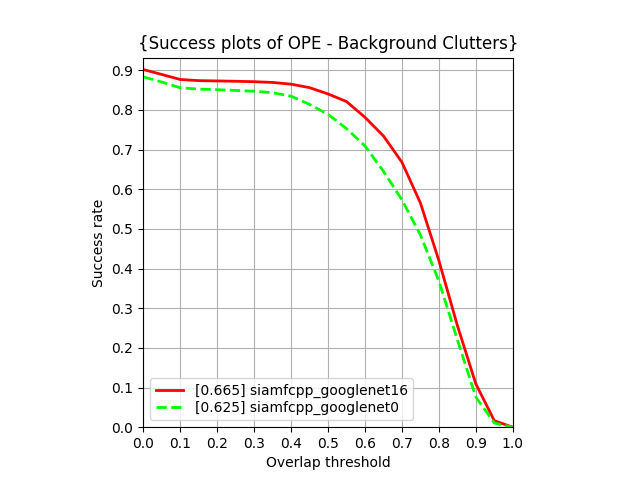
\includegraphics[width=0.33\textwidth]
	{Img/MTP/otb2015/success_Background Clutters.png}
}\\
\subfloat[]{
	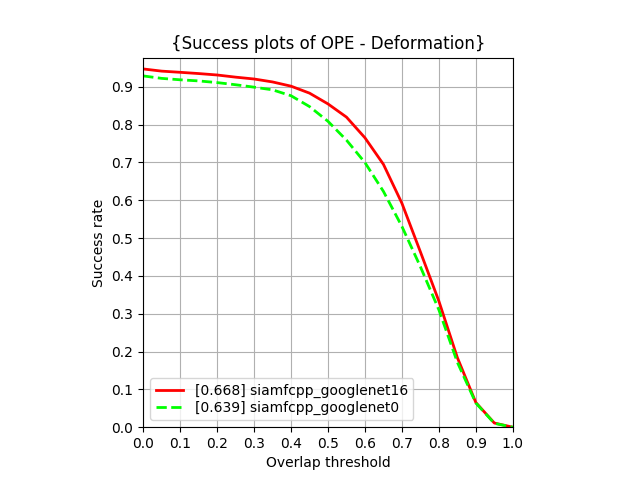
\includegraphics[width=0.33\textwidth]
	{Img/MTP/otb2015/success_Deformation.png}
}
\subfloat[]{
	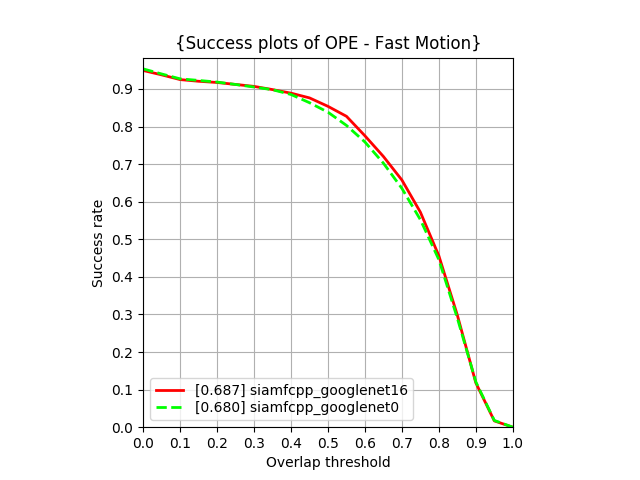
\includegraphics[width=0.33\textwidth]
	{Img/MTP/otb2015/success_Fast Motion.png}
}
\subfloat[]{
	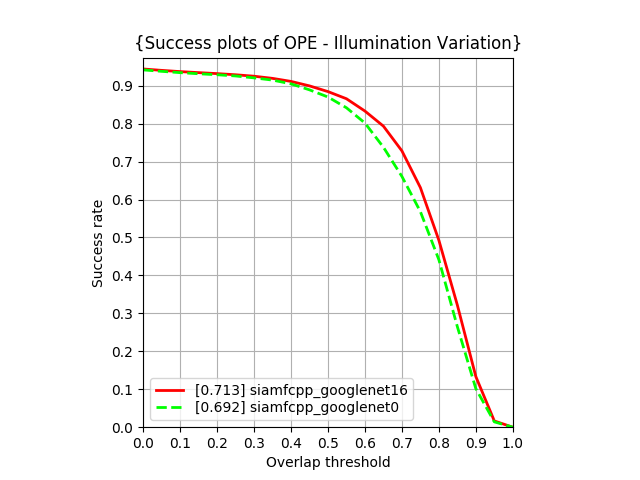
\includegraphics[width=0.33\textwidth]
	{Img/MTP/otb2015/success_Illumination Variation.png}
}\\
\subfloat[]{
	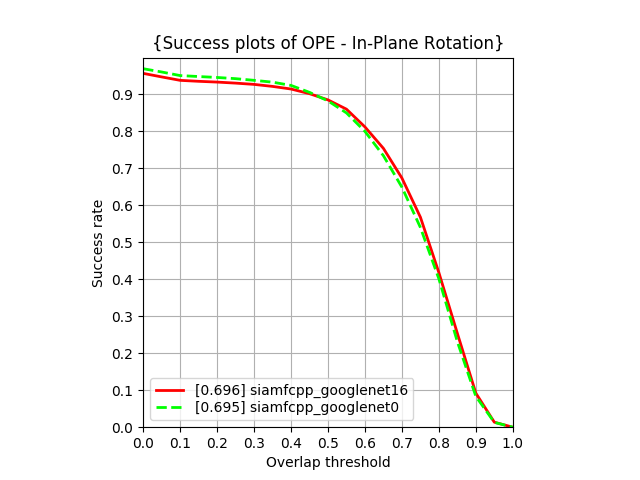
\includegraphics[width=0.33\textwidth]
	{Img/MTP/otb2015/success_In-Plane Rotation.png}
}
\subfloat[]{
	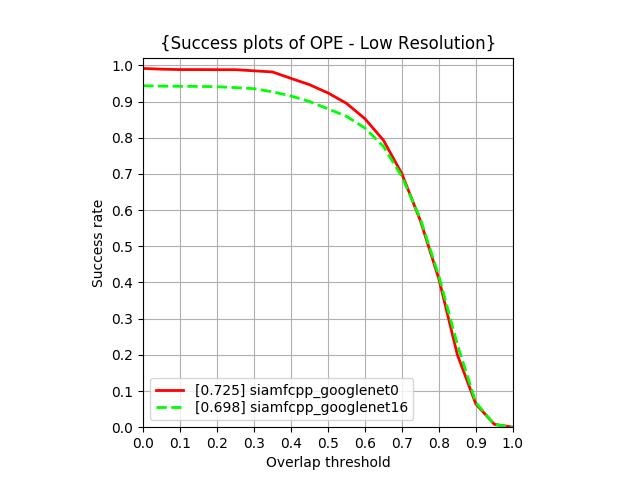
\includegraphics[width=0.33\textwidth]
	{Img/MTP/otb2015/success_Low Resolution.png}
}
\subfloat[]{
	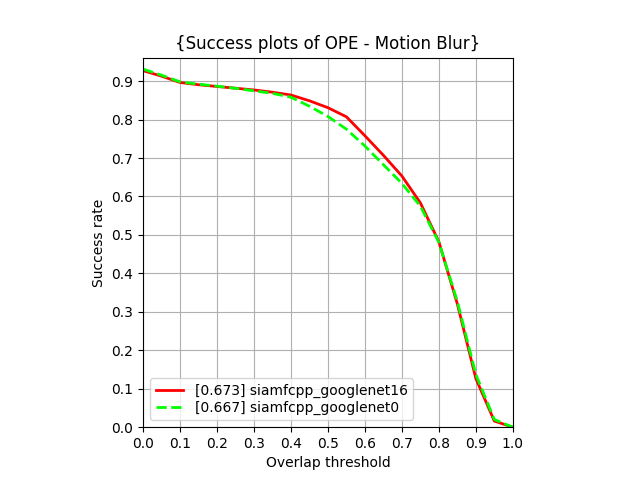
\includegraphics[width=0.33\textwidth]
	{Img/MTP/otb2015/success_Motion Blur.png}
}
\end{center}
   \caption{OTB 各属性成功图。}
\end{figure*}
\fi

\textbf{OTB2015} 我们使用成功率来评估跟踪器在 OTB2015 上的性能。成功率取决于预测边界框和真实边界框的交并比。我们将本章提出的方法与各种跟踪算法进行了比较,包括 ECO \cite{danelljan2017eco},MDNet \cite{MDNet},SiamRPN++ \cite{SiamRPN++},ATOM \cite{danelljan2019atom} 和 SiamFC++\_GoogLeNet \cite{SiamFC++}。模板更新的迭代次数设置为 16。结果显示在表 \ref{table:otb} 中。在成功率方面,我们的跟踪器比在线跟踪器 ATOM 高出 2.8%,这证明了我们方法的强大模型自适应能力。

\textbf{VOT2018} 我们将我们的方法与 RCO \cite{kristan2018sixth},UPDT \cite{bhat2018unveiling},SiamRPN \cite{SiamRPN},MFT \cite{kristan2018sixth},LADCF \cite{kristan2018sixth},ATOM \cite{danelljan2019atom},SiamRPN++ \cite{SiamRPN++},SiamFC++\_AlexNet \cite{SiamFC++} 和 SiamFC++\_GoogLeNet \cite{SiamFC++} 在 VOT2018 上进行了比较。使用鲁棒性和精确度来比较跟踪器。鲁棒性表示跟踪失败的次数,而精确度表示跟踪器预测边界框与真实边界框之间的平均重叠。两种度量方式被合并为单个评价指标)——预期平均重叠(EAO)分数。模板更新的迭代次数设置为 2。如图 \ref{fig:eao} 所示,本章提出的跟踪器性能超越了所列出的其他跟踪器。

\textbf{GOT-10k} 我们将平均重叠(AO)分数用作 \cite{GOT-10k} 的性能指标。我们将本章提出的方法与 CF2 \cite{CF2},ECO \cite{danelljan2017eco},CCOT \cite{CCOT},GOTURN \cite{GOTURN},SiamFC \cite{SiamFC},SiamFCv2 \cite{valmadre2017end},ATOM \cite{danelljan2019atom},SiamFC++\_AlexNet \cite{SiamFC++} 和 SiamFC++\_GoogLeNet \cite{SiamFC++} 在该数据库上进行比较。模板更新的迭代次数设置为 2。在图 \ref{fig:got10k} 中可以发现,与列出的跟踪器相比,本章提出的算法具有更好的跟踪性能。

\textbf{TrackingNet} 我们将本章提出的方法与 SiamFC \cite{SiamFC},ECO \cite{danelljan2017eco},MDNet \cite{MDNet},SiamRPN++ \cite{SiamRPN++},ATOM \cite{danelljan2019atom},SiamFC++\_AlexNet \cite{SiamFC++} 和 SiamFC++\_
GoogLeNet \cite{SiamFC++} 进行比较。模板更新的迭代次数设置为 32。表 \ref{tabel:trackingnet} 显示,我们的跟踪器在精确度和标准化精确度方面表现最佳,同时保持了较高的成功率。

\subsection{对初始帧噪声的鲁棒性分析}

%%%%%%%%%%%%%%%
\begin{table}[t]
\centering
\caption{使用嘈杂的初始帧在 OTB2015 上的性能。}
\begin{tabular}{c c c c c}
\toprule
\multicolumn{3}{c}{噪声系数} & \multicolumn{2}{c}{成功率得分} \\
\cmidrule(lr){1-3} \cmidrule(lr){4-5}
$\gamma_1$ & $\gamma_2$ & $\gamma_3$  & SiamFC++\_GoogLeNet & 本章算法  \\
\midrule
0.57  &	1.6	 & 0.93	& 67.3    & 69.5 \\
%0.82  & 1.1  & 0.82 & 65.9    & 67.2 \\
0.88  & 0.22 & 0.86 & 65.7    & 68.0 \\
0.88  & 0.43 & 0.77 & 64.1    & 64.4 \\
0.92  & 0.98 & 0.82 & 65.6    & 66.6 \\
0.98  & 0.83 & 0.84 & 66.5    & 67.9 \\
1.0   & 0.81 & 0.79 & 65.3    & 66.0 \\
1.1   &	1.9  & 0.90	& 67.6    & 68.8 \\
1.2   & 0.70 & 0.79 & 65.7    & 66.6 \\
1.3   & 1.3  & 0.77 & 64.9    & 65.8 \\
1.5   & 0.19 & 0.79 & 64.8    & 66.3 \\
1.5   & 1.3  & 0.86 & 66.7    & 68.0 \\
\bottomrule
\end{tabular}
\label{table:noise}
\end{table}
%%%%%%%%%%%

\iffalse
To verify the contribution of the proposed model adaptation method, we compare our tracker with the baseline SiamFC++\_GoogLeNet \cite{SiamFC++} on 4 challenging tracking datasets. In comparison with the baseline tracker on OTB2015, our tracker improves the success score by 1.4\%. On VOT2018, our tracker outperforms the baseline tracker by 1.2\% in terms of EAO. On GOT-10k, our tracker improves the AO score by 1.0\%. On TrackingNet, our tracker outperforms the baseline tracker by 1.7\% in terms of the normalized precision score. All these consistent improvements highlight the effectiveness of the proposed model adaptation method.
\fi

为了研究本章提出的模型自适应方法在第初始帧与后续帧相比有噪声的情况下的鲁棒性,我们通过以下方式在第一帧中添加三种噪声:更改图像亮度,应用高斯模糊以及使用不准确的真实边界框注释。我们用 $\gamma_1 \in [0.5, 1.5]$ 表示亮度变化系数,用 $\gamma_2 \in [0, 2]$ 表示模糊半径系数,用 $\gamma_3 \in [0.75, 1]$ 表示不准确的第一帧边界框注释和真实边界框注释之间的边框重叠交并比(IoU)。我们随机采样 $\gamma_1, \gamma_2$ 和 $\gamma_3$,并在 OTB2015 上对基线跟踪器和我们的跟踪器都运行了 10 次(见表 \ref{table:noise})。与 SiamFC++\_GoogLeNet \cite{SiamFC++} 相比,我们的跟踪器在不同的噪声水平下始终表现更好,这表明我们的跟踪器对嘈杂的初始帧具有鲁棒性。%the first frame noise.

%%%%%%%%%%%%%%%%
\begin{table}[t]
%\renewcommand\arraystretch{0.8}
\centering
\caption{OTB2015 在 11 种属性下对成功率进行比较。}
\resizebox{\textwidth}{!}{%
\begin{tabular}{c c c c c c c c c c c c}
\toprule
跟踪器 & BC & DEF & FM            & IV            & IPR           & LR    & MB    & OCC   & OPR   & OV    & SV    \\
\midrule
基线算法  &  62.5 & 63.9 & 68.0          & 69.2          & 69.5          & \textbf{72.5}  & 66.7 & 60.9 & 66.9 & 55.8 & 68.4 \\
本章算法        & \textbf{66.5} & \textbf{66.8} & \textbf{68.7} & \textbf{71.3} & \textbf{69.6} & 69.8  & \textbf{67.3} & \textbf{62.5} & \textbf{68.4} & \textbf{57.1} & \textbf{69.8} \\
\bottomrule
\end{tabular}
}
\label{table:attr}
\end{table}
%%%%%%%%%%%

\subsection{基于 OTB 数据集不同属性的评测结果分析}
为了对跟踪性能进行进一步分析,我们还通过对 OTB2015 数据集的序列进行基于属性的比较来证明我们算法的优势(请参见表 \ref{table:attr})。在 OTB2015 中,每个序列都具有 11 种不同的属性,即:背景混杂(BC),形变(DEF),快速运动(FM),照明变化(IV),平面内旋转(IPR),低分辨率(LR),运动模糊(MB),遮挡(OCC),平面外旋转(OPR),目标出画面(OV)和缩放尺度变化(SV)。在 11 个属性中,与 SiamFC++\_GoogLeNet \cite{SiamFC++} 相比,本章提出的跟踪器在 10 个属性上具有更好的性能,这证明了其在挑战性跟踪场景(例如照明变化和运动模糊)中的鲁棒性。

%%%%%%%%%%%%%%%%%%%%
\section{本章小结}
在本章中,我们提出了一种用于孪生跟踪器的新型模型自适应方法,可实现高速准确的跟踪。我们表明,在视觉目标跟踪中具有挑战性的模型适应任务可以使用第一帧中的目标真实标注框,通过简单地操纵模板图像的像素来实现。我们的模型自适应方法是可插拔的,因为它不会改变基本跟踪器的总体架构。在四个目标跟踪基准上的大量实验结果证明了所提出的模型自适应方法的有效性。